% =====================================================================
%  The Dose Train is the Identification Experiment
%  Build:  make paper     (or: latexmk -pdf main.tex)
%  Figures are produced by src/; run `make figures` first.
% =====================================================================
% Pass the class option `draft` to include the claim-register appendix:
%     make paper-draft
% or  pdflatex "\PassOptionsToClass{draft}{article}% =====================================================================
%  The Dose Train is the Identification Experiment
%  Build:  make paper     (or: latexmk -pdf main.tex)
%  Figures are produced by src/; run `make figures` first.
% =====================================================================
% Pass the class option `draft` to include the claim-register appendix:
%     make paper-draft
% or  pdflatex "\PassOptionsToClass{draft}{article}\input{main}"
% The default build omits it.
\documentclass[11pt,a4paper]{article}

% `draft` is article's own option, and it is detected here by its effect
% rather than by reading the option list, so that it is seen whether it is
% written into \documentclass above or handed over with \PassOptionsToClass
% on the command line. article's draft mode sets \overfullrule; nothing else
% in this preamble does.
\makeatletter
\newif\ifshowregister
\ifdim\overfullrule>\z@ \showregistertrue \fi
\makeatother

% Both of article's draft-mode effects are now undone, so the register build
% is otherwise identical to the default one: no rules in the margin, and no
% blanked figures. graphicx is pulled in by tikz, so its option has to be
% passed rather than given at load time, and passed before any package loads.
\overfullrule=0pt
\PassOptionsToPackage{final}{graphicx}

\usepackage[T1]{fontenc}
\usepackage[utf8]{inputenc}
%\usepackage{lmodern}
\usepackage[margin=2.1cm]{geometry}
\usepackage{changepage}
\usepackage{amsmath,amssymb,amsthm}
\usepackage{booktabs}
\usepackage{longtable}
\usepackage{array}
\usepackage{tikz}
\usetikzlibrary{arrows.meta,positioning,shapes.geometric,calc}
\usepackage{graphicx}
\graphicspath{{../results/figures/}{results/figures/}}
\usepackage{caption}
\usepackage[colorlinks=true,linkcolor=black,citecolor=black,urlcolor=blue]{hyperref}

% Bibliography. refs.bib is GENERATED by tools/fetch_refs.py from
% paper/refs.sources; do not edit it.
\usepackage[backend=biber, style=numeric-comp, sorting=none,
            maxbibnames=6, minbibnames=3, giveninits=true]{biblatex}
\addbibresource{refs.bib}
\usepackage{enumitem}
\usepackage{xcolor}

\definecolor{accent}{RGB}{122,47,47}
\definecolor{soft}{RGB}{244,242,238}

\newtheorem{assumption}{Assumption}
\newtheorem{remark}{Remark}
\newtheorem{proposition}{Proposition}

\newcommand{\thc}{\theta_{\mathrm{crit}}}
\newcommand{\spk}{s_{\mathrm{peak}}}



\title{\textbf{The Dose Train is the Identification Experiment:\\
Estimating Residual Enzymatic Capacity in Propionic Acidemia}}
\author{Guido Putignano\\[2pt]
  \normalsize\itshape \textnormal{[affiliation]}\\
  \normalsize\texttt{[corresponding author e-mail]}}
\date{\today}

\begin{document}
\maketitle

\begin{abstract}
\noindent
The clinical decision in mRNA enzyme replacement for propionic acidemia is a dosing
interval. It is set by the patient's residual enzymatic capacity, which is never measured.
We ask how much of it the records can recover.

Over the narrow band a stable patient's marker visits, total clearance is indistinguishable
from a straight line at assay resolution. The capacity survives only in that line's
intercept, which the band reaches by extrapolation and which carries the half-saturation
constant with it. Its location is unresolved across two orders of magnitude; its relative
precision is not.

The decision survives this. The safety margin is linear along the unresolved direction
where the capacity is quadratic in it. Its sign is therefore fixed, except for illness
amplitudes inside a window we compute.

The capacity itself is not recovered, and the design that would recover it fails in two ways
at once. The precision of the intercept has a floor set by the number of perturbation events
alone, which no width of band beats: at six events and a load recorded to $2\%$, that floor
is $53\%$, and $20\%$ precision needs forty-three events. Resolving the curvature that
separates the two channels needs the marker carried to between three and five times its
operating level, and the perturbations available in a chart move the patient the other way.

The conflation the analysis turns on has been measured directly. Propionate oxidation
assayed by breath test is near-identical in patients whose serum markers differ widely, and
repeats at a coefficient of variation of $6.9\%$ in controls and $12.8\%$ in
patients~\cite{breath_test_mma}. Capacity and marker level are different quantities, and the
second does not report the first.

A selective perturbation identifies the system formally, and the determinant turns on the
excursion and the half-saturation constant rather than on which channel produced it, so the
question can be posed on carnitine and answered for the therapy. That interchangeability
holds given the half-saturation constant and fails without it, by orders of magnitude:
carnitine buys the excursion, and only a perturbation on the enzymatic channel, or an
excursion reaching the half-saturation level itself, buys the curvature.
\end{abstract}

\vspace{0.5em}
\hrule
\vspace{1.5em}

%==========================================================================


\vspace{0.6em}
\noindent\textbf{Keywords.} structural identifiability; optimal experimental
design; sampling schedule; enzyme replacement; propionic acidemia; pharmacokinetic
excitation; Cram\'er--Rao bound.

\vspace{0.5em}\hrule\vspace{1.5em}

% The main text is written to four claims and nothing wider; see Section 1.
% The biological background, the full dynamic model and its equilibrium
% reduction, and the local model's derivation were moved to the appendix in
% the phase 3 compression. Nothing was deleted and every label came with the
% text, so every cross-reference into that material still resolves.
\section{The question}
\label{sec:question}
%==========================================================================

Propionic acidemia is an autosomal recessive disorder of propionate metabolism. Four amino
acids, odd-chain fatty acids and propionate from intestinal flora converge on
propionyl-CoA, which propionyl-CoA carboxylase (PCC) carboxylates onward into the
tricarboxylic acid cycle. When PCC is defective the intermediate accumulates, spills into
alternative routes, and periodically overwhelms them: the patient decompensates, with
hyperammonaemia and metabolic acidosis. Decompensations are frequent, $49$ of $50$
participants in a natural history cohort reported at least one, at a mean annualised
frequency of $1.0$~\cite{natural_history}, % C08
and they carry the neurological damage that defines the disease's course.

mRNA enzyme replacement supplies PCC transiently~\cite{trial_phase12}. % C16
The clinical decision it creates is a \emph{dosing interval}, and the interval is set by a
quantity nobody measures: the patient's residual enzymatic capacity, written $\theta$
throughout. A patient with more residual capacity needs less frequent replacement.

This note asks a narrow question and answers it. Given a clinical record of the
kind the disease actually generates (a marker series, a dosing diary, a dietary record) \emph{can $\theta$ be identified, and does identifying it decide anything?} The answer
is in four parts, and the second is the one that determines what a protocol should do.

\begin{enumerate}[leftmargin=*, itemsep=3pt]
\item \textbf{The dose train is the identification experiment, and it is already being
run.} The therapy is administered on a fixed biweekly schedule and read as treatment; it is
also a known, exogenous, selective input on exactly the parameter in question, and it
supplies forty-two times the excitation the marker's own excursions do. That is what makes
$\theta$ identifiable: monthly outpatient draws across dose cycles reach $17\%$ over two
years. One scheduling choice destroys it, and it is the choice a protocol would make for
convenience: sampling on dosing days, or at any multiple of the dose interval, costs a
factor of twenty-two, and moving the schedule half a day recovers it
(Sections~\ref{sec:excitation} and~\ref{sec:designsec}).

The obstruction is why this works rather than a finding in its own right. The model is
globally structurally identifiable, so the information is in the system; what a monthly
record loses is the transient. On the quasi-steady locus that remains, the degeneracy has
an exact closed form, a rank-one identity in capacity, affinity and the unrecorded load,
and that identity names the input that closes it. The corollary is a limit on reach
rather than on precision: nothing but the dose train supplies enough excitation, so the
design applies to patients receiving the therapy and to no one else
(Section~\ref{sec:whoto}).
\item \textbf{Identifying $\theta$ does not decide the dosing interval.} The decision is
usually posed as the sign of $\mu = \theta - \thc$ against a critical capacity. That
threshold is not a measured quantity: it is defined through two chosen constants, and
across their defensible range it moves by a factor of $24$ and the sign flips for the same
patient with perfect data (Section~\ref{sec:decision}).
\item \textbf{The threshold framing is itself doubtful.} The only endpoint evidence
available reports a smooth dose--response and no threshold at all. This note records that
as a finding rather than adopting a replacement estimand, for reasons given in
Section~\ref{sec:decision}.
\item \textbf{And capacity stops being recoverable exactly where it matters most.} Above
roughly three to four times the managed marker level, two patients differing tenfold in
residual capacity are indistinguishable, which is the severely affected population
(Section~\ref{sec:scope}).
\end{enumerate}

What this note is not. It is a statement about identifiability, a property of a
model and a design together. It is not a statement about patients, and
Section~\ref{sec:discussion} says plainly where the model's own analysis questions its
validity. The biological background, the disease's clinical course and the argument for
treating $\theta$ as the decision variable are in the supplement, \S S1.

\vspace{0.5em}
\hrule
\vspace{1em}

%==========================================================================

\section{Model and methods}
\label{sec:model}
%==========================================================================

\emph{This section fixes the model, the parametrisation and the numerical conventions every
result below depends on. One model is used throughout, at three levels of detail; the
derivations, the alternative hypotheses that were rejected and the checks behind each step
are in the supplement, \S S1, and Section~\ref{sec:discussion} says what one model at three
levels of detail does and does not license.}

\subsection{Notation}

\begin{adjustwidth}{-1.0cm}{-1.0cm}
\begin{table}[htbp]
\centering
\footnotesize
\caption{\label{tab:notation}Notation, once, in one place. Values and sources are in
Table~\ref{tab:params}.}
\begin{tabular}{@{}ll@{\hskip 2em}ll@{}}
\toprule
$m$ & the plasma marker, 3-HP & $\bar m$ & the operating point, and the sample mean \\
$L(t)$ & recorded propiogenic load & $L_0$ & its \emph{unrecorded} component, unknown \\
$\theta$ & residual capacity, absorbing $V_{\max}$ & $\Delta(t)$ & therapeutic increment,
scheduled \\
$K_m$ & half-saturation, at the plasma level & $u_c(t)$ & recorded carnitine dose \\
$k_e$ & alternative clearance & $\kappa$ & its gain onto $k_e$, never assigned \\
$g(m)$ & $m/(K_m+m)$, the saturation & $\alpha(m)$ & the alternative channel, general \\
$C(m)$ & total clearance & $(a,b)$ & its affine fit over the band \\
$\Delta$ & \textbf{full} width of the band & $r$ & its fold range, $m_{\max}/m_{\min}$ \\
$\varphi(m)$ & $K_m/(K_m+m) = 1-g(m)$ & $E$ & the excitation, $\varphi$'s drop across a
band \\
$\thc$ & critical capacity & $\mu$ & the margin $\theta - \thc$, whose \emph{sign} decides \\
$\mtol$ & tolerable level, a convention & $\spk$ & illness amplitude, as a fold of baseline \\
\bottomrule
\end{tabular}
\end{table}
\end{adjustwidth}


\subsection{The dynamic model}
\label{sec:parent}

The metabolite the clinic measures is written $m$. Its balance is
\begin{equation}
\dot m \;=\; L(t) + L_0 \;-\; \bigl(\theta + \Delta(t)\bigr) g(m) \;-\; \alpha(m),
\qquad g(m) = \frac{m}{K_m + m},
\label{eq:parent}
\end{equation}
with $L$ the \emph{recorded} component of the propiogenic load, $L_0$ its unrecorded
component carried as an unknown constant, $\Delta$ the therapeutic increment known from
the dosing record, and $\alpha$ an alternative clearance route: in propionic acidemia,
principally conjugation to carnitine and renal loss of the conjugate. Carrying $L_0$ as an
unknown rather than assuming it away is what makes the identification problem well posed
at all.

The parametrisation is pinned: $\theta$ \emph{absorbs} the maximal velocity, so it
\emph{is} the patient's residual $V_{\max}$ rather than a fraction of a population one.
Carrying the two separately as $V_{\max}\theta\,g(m)$ adds a parameter no excursion
separates, since only the product multiplies $g$; splitting them needs an anchor outside
the marker, and a $1$-$^{13}$C-propionate breath test is what such an anchor looks
like~\cite{breath_test_mma}. % C48

\paragraph{Why $\alpha$ is not a rate constant.} Elimination proceeds by conjugating
propionate with carnitine, one molecule of carnitine per molecule eliminated, excreted
with the product; in two patients with propionic acidemia and two with methylmalonic
aciduria, urinary free carnitine was decreased while short-chain acylcarnitines, mostly
propionylcarnitine, were increased~\cite{carnitine_excretion_pa}. % C41
Stoichiometric consumption alone would give a ceiling rather than a decline: promote
carnitine to a state $c$ with constant replenishment, and if conjugation is its only exit
then $\dot c = 0$ fixes the conjugation flux at every $m$. What is missing is a reason for
the flux to vanish as the metabolite does and a reason for it to decline, and one mechanism
supplies both. Carnitine is recovered from the glomerular filtrate by a renal transporter
that acylcarnitines share, and in a transporter solubilised from renal apical brush-border
membrane and reconstituted into liposomes the most effective inhibitors were
acylcarnitines~\cite{octn2_renal_transport}. % C42
Propionylcarnitine rises with the metabolite, so the fraction of filtered carnitine
recovered falls as the metabolite accumulates: the free pool has a second exit, and that
exit grows with $m$. Writing $c(t)$ for available carnitine,
\begin{equation}
\begin{aligned}
\dot m &= s(t) \;-\; \theta\, g(m) \;-\; k\, c\, \frac{m}{K_c + m}, \\[2pt]
\dot c &= R_0 \;-\; k\, c\, \frac{m}{K_c + m} \;-\; \delta(m)\, c,
\qquad \delta(m) = \delta_0\left(1 + \frac{m}{M_i}\right),
\end{aligned}
\label{eq:twostate}
\end{equation}
with $K_c$ the half-saturation of the conjugation step, $\delta_0$ the basal rate of
non-conjugative loss, $M_i$ the metabolite level at which competition doubles it, and $R_0$
constant. The conjugation term is the one the two equations share, entering both with the
same coefficient, which is the one-to-one stoichiometry; they are otherwise not symmetric,
because carnitine has a second exit that propionate does not. The supplement, \S S1, draws
the system as a block diagram and works through the positive feedback it creates.

\subsection{The equilibrium reduction}
\label{sec:reduction}

\textbf{The carnitine state is not fast relative to the metabolite, and no separation of
timescales is needed to justify eliminating it.} The comparison that would be needed is
carnitine against the \emph{marker}, and it runs the wrong way: at the model's own $k$ the
carnitine time constant is $0.92$~d against the marker's $0.81$~h, slower by a factor of
$27$, and published human kinetics put whole-body carnitine turnover at $38$ to $119$~h
with a rapidly equilibrating compartment at $2$ to $3$~h (Rebouche, \emph{Ann.\ N.\ Y.\
Acad.\ Sci.} 2004), slower on either reading.

What justifies the reduction is algebraic and needs no separation at all. $\alpha$ is
\emph{defined} by solving $\dot c = 0$, and $\dot c = 0$ holds exactly at any fixed point,
so at equilibrium the two formulations are one equation rearranged, whatever the timescales
do, and everything this paper computes from the parent is computed at equilibrium. Solving
$\dot c = 0$ in \eqref{eq:twostate} for $c$ and substituting gives that flux in closed form,
\begin{equation}
\alpha(m) \;=\; R_0\,\frac{u(m)}{u(m) + \rho(m)},
\qquad u(m) = \frac{m}{K_c+m},
\qquad \rho(m) = \rho_0\left(1 + \frac{m}{M_i}\right),
\label{eq:alphaqss}
\end{equation}
with $\rho_0 = \delta_0/k$. The conjugation rate constant $k$ enters only through that
ratio and cancels from the reduced clearance, exactly. \textbf{It does not follow that $k$
is a free scale}: $k$ alone sets the carnitine relaxation rate,
$\tau_c = 1/(k[u(m) + \rho(m)])$, so it sets the reduction's validity \emph{off}
equilibrium even though it cancels from the curve, and what assuming it costs is bounded in
the $k$ row of the full registry, supplement \S S2, rather than argued away.

Setting $\dot m = 0$ gives the equilibrium reduction, which is what a steady-state fit to a
clinical record actually estimates. Its solutions are an attractor and a separatrix, and the
fold at which the two collide defines the critical capacity $\thc$: below it a sufficiently
large load leaves the system with no equilibrium at all, which is what a decompensation is
in this model. \textbf{Integrating \eqref{eq:twostate} and watching it settle on the
reduced attractor to fourteen digits is not evidence for the reduction}: it is the identity
above, so it cannot fail at any parameter value and reports nothing about the premise. The
divergence from above the separatrix needs a qualification too. Started \emph{on} the slow
manifold a trajectory a tenth of a per cent above the separatrix does run away, but started
off it, with carnitine at its pre-perturbation value, the same trajectory can return to the
attractor, so the reduced separatrix is a lower bound on the true basin and not the basin.
The intrinsic definition of $\thc$, the fold, and the comparison against the alternative
hypothesis with a ceiling instead of a fold are in the supplement, \S S1.

\subsection{The local identification model}
\label{sec:localmodel}

Linearising $\alpha \to k_e m$ gives the \emph{local identification model}, which is the one
every design calculation below uses:
\begin{equation}
\dot m \;=\; L(t) + L_0 \;-\; \bigl(\theta + \Delta(t)\bigr) g(m) \;-\; k_e\, m.
\label{eq:local}
\end{equation}

\begin{figure}[htbp]
\centering
\resizebox{0.90\linewidth}{!}{%
\begin{tikzpicture}
\node[mpool] (m) at (0,0) {$m$\\[1pt]\scriptsize\mdseries accumulated\\metabolite};
\node[mlabel] (in) at (-3.6,0) {$s(t)$};
\draw[mar] (in) -- (m);
\node[msmall] at (-2.4,0.42) {load};

\node[menzy] (enz) at (-2.3,-2.7) {$\theta\, g(m)$\\{\scriptsize saturating}};
\channelglyph{(-3.55,-4.15)}{green!45!black}{s}

\node[malt] (alt) at (2.3,-2.7) {$k_e\, m$\\{\scriptsize linear}};
\channelglyph{(1.15,-4.15)}{blue!55!black}{l}

\draw[mar] (m.south) -- ++(0,-0.55) -| (enz.north);
\draw[mar] (m.south) -- ++(0,-0.55) -| (alt.north);

\node[msmall] (o1) at (-2.3,-5.0) {eliminated};
\node[msmall] (o2) at (2.3,-5.0) {eliminated};
\draw[mar] (enz) -- (o1);
\draw[mar] (alt) -- (o2);

\node[mlabel, green!45!black] (thr) at (-6.6,-2.7) {therapy\\$\Delta(t)$};
\draw[mar, green!45!black] (thr) -- (enz);
\node[mlabel, blue!55!black] (carn) at (6.6,-2.7) {carnitine\\$u_c(t)$};
\draw[mar, blue!55!black] (carn) -- (alt);
\end{tikzpicture}}
\caption{The local identification model \eqref{eq:local} as a block diagram. One pool $m$,
filled by the load $s(t)$ and drained by two channels. The enzymatic channel saturates at
$\theta$; the alternative channel is linear in $m$, and in the \emph{unforced} model that
difference in shape is the only thing separating them. A known input that varies and rides
on one channel alone is a second and independent separator. The two selective inputs are
drawn together because, \emph{at fixed} $K_m$, they are interchangeable: carnitine acts on
$k_e$ and is recorded for every patient, the therapy acts on $\theta$ and is administered on
the published biweekly schedule, and at fixed $K_m$ the identification problem cannot tell
which one moved the patient. With $K_m$ free they are not interchangeable (supplement, \S S1); the design of Section~\ref{sec:designsec} uses the therapy.}
\label{fig:blockA}
\end{figure}


\begin{figure}[htbp]
\centering
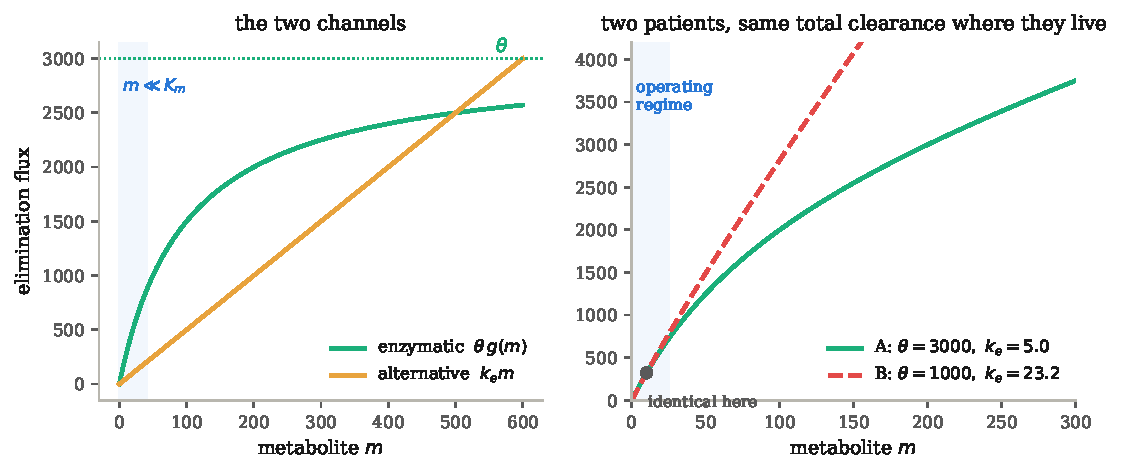
\includegraphics[width=\textwidth]{fig_A1_channels.pdf}
\caption{Left: the two elimination channels. The enzymatic term saturates at $\theta$ while
the alternative term does not, and this difference in functional form is the only thing
distinguishing them in the unforced model. In the shaded band, where clinically stable
patients are maintained, both are approximately linear, which is the difficulty the rest of
this paper is about. Right: two patients agreeing in \emph{both} the value and the slope of
total clearance at the operating point, differing only at second order. They differ
threefold in enzymatic capacity and carry different $K_m$, and no affine fit over a band
around that point tells them apart.}
\label{fig:A1}
\end{figure}


\paragraph{Why the local model is used.} It is not a reduction of the parent. The tangent
to the parent's clearance curve carries an extra term in its intercept, and at the
illustrative constants that term is $374$ against the enzymatic term's $61$, so the
alternative channel owns six-sevenths of an intercept the residual capacity was supposed to
carry. The local model is therefore a different hypothesis about one term, kept because it
is the most favourable case for identification rather than because it approximates
anything, and that is what the conclusion needs: the degeneracy this paper is about appears
in the favourable structure and disappears in the awkward one, so it is not an artefact of a
bad approximation. At matched parameter count the parent carries a degenerate family of the
same dimension, admissible over a sixteen-fold range in $K_m$ and if anything harder to
reject. What closes such a family, in either model, is an independent channel being known,
not curvature in $\alpha$. The reduction hierarchy is verified symbolically and numerically
(supplement, \S S2).

\subsection{Assumptions and their status}
\label{sec:assumed}

\begin{adjustwidth}{-1.0cm}{-1.0cm}
\scriptsize
\def\paramslabel{tab:params}
\def\paramscaption{The constants this paper reasons about, and what each rests on. Three
are from the literature and the rest are chosen for illustration, against what the last
column says. Each row also carries what \emph{kind} of quantity it is, which is a
different question from where it came from, and the species its evidence comes from where
there is one. \textbf{Some conclusions do depend on values in this table}, and the three
that decide a result are priced in the text below. The full registry is \S S2 of the
supplement, which is the authority; this is a selection from it.}
\input{../results/tables/tab_params_compact}
\end{adjustwidth}


\paragraph{The three rows that decide a result, and what each is worth.} Most of the table
is illustrative in the harmless sense that every conclusion is stated relative to it. Three
rows are not.

\emph{Capacity.} The identifiability results do not turn on $\theta = 3000$, but two
conclusions do. The supplement's local-model section flips a qualitative conclusion across
it, the anchor attenuating at $3000$ and amplifying at the parent model's $300$, and by
Section~\ref{sec:scopeprec} the design's own precision does too.

\emph{Capacity in the disease.} On the monthly record $\operatorname{sd}(\ln\hat\theta)$ is
$0.1699$ at nominal capacity, $1.5830$ at $10\%$ of nominal and $3.0673$ at $5\%$, against
a target of $0.20$. The gate holds only for $\theta$ between $2472$ and $18814$, which is
$82\%$ to $627\%$ of nominal, so the disease sits a factor of $16$ below the band. This is
the row that says who the paper is about, and it is the reason the precision above is an
illustration rather than the result.

\emph{Half-saturation.} This is the tightest cost in the local model after the increment.
Holding the patient managed at $\bar m$ and re-solving the load, the ordinate noise and the
load-bias prior at each $K_m$, $\operatorname{sd}(\ln\hat\theta)$ runs $0.0507$ to $1.3608$
over $K_m$ from $5$ to $1000$~$\mu$M, a factor of $26.8$. It is $0.1699$ at the
illustrative $100$ and crosses the target at $K_m = 124$, so the design has a factor of
$1.24$ of headroom; at the in vitro value the $K_m$ row declines to use, $290$~$\mu$M, it
would be $0.4158$. That headroom is smaller than it reads: across twenty-four intake
records the spread is $0.1684$ to $0.1709$ at $K_m = 100$ and $0.1987$ to $0.2010$ at
$K_m = 124$, so the crossing straddles the target and which side of it a given record falls
on is not settled by the median.

Two consequences of that table are load-bearing and are stated here rather than left to be
inferred.

\begin{remark}[No value of $K_m$ is imported, and none is needed]
\label{rem:no_km}
The in vitro Michaelis constant of PCC is for propionyl-CoA inside the mitochondrion. The
$K_m$ of \eqref{eq:local} is for a plasma marker that is neither that molecule nor in that
compartment, and the two are not interchangeable, so no literature value is used. The
results below do not need one: a prior on $\ln K_m$ twenty times looser than the module's
own changes $\operatorname{sd}(\ln\hat\theta)$ in the fourth decimal, and removing it
entirely changes nothing at all (Section~\ref{sec:designsec}).
\end{remark}

\begin{remark}[The marker, and the observation model both markers need]
\label{sec:marker}
Plasma 3-hydroxypropionate is used. It is the one marker with an endpoint association: a
$50\%$ lower concentration carries a decompensation rate ratio of $0.7$ ($95\%$ CI
$0.6$--$0.9$, $p<0.01$)~\cite{natural_history}, % C49
where 2-methylcitrate has none ($1.0$, $0.7$--$1.3$), and it is not a carnitine conjugate,
so carnitine supplementation does not raise it as it raises C3. But no marker is the PCC
substrate. 3-HP is an overflow metabolite downstream of accumulated propionyl-CoA, and so
is 2-MC. Writing either as the $m$ of \eqref{eq:parent} assumes it tracks the substrate
monotonically: an assumption required identically for either choice, not testable from the
published data, and named first among the limits in Section~\ref{sec:discussion}.
\end{remark}

\subsection{Numerical methods}
\label{sec:numerics}

Every computed trajectory uses an adaptive stiff-capable solver (\texttt{LSODA} or
\texttt{Radau}) at relative tolerance $10^{-8}$ or tighter, and the estimator of
Section~\ref{sec:collapse} does not integrate at all: it uses the closed-form quasi-steady
level of \eqref{eq:alphaqss}. Two tests guard the integration, one halving the step and
asserting the answer moves by less than $10^{-6}$ relative, the other asserting that an
integrated steady state equals the closed-form equilibrium reduction to the same tolerance.
\textbf{Neither measures the validity of the carnitine reduction}, because the first
integrates the local model and the second integrates the \emph{reduced} system and compares
it against the algebraic root of the same reduced clearance, so the two-state system appears
in neither. What licenses the reduction is the identity of \S\ref{sec:reduction}, and what
bounds its cost off equilibrium is the $k$ row of the supplement's registry, \S S2.

Every stochastic result uses \texttt{numpy.random.default\_rng} with an explicit seed named
at the call site, and each quoted precision is a median over $24$ intake records with its
range beside it unless stated otherwise. Fitted ensembles are cached on
$(\text{design}, \sigma, \mathrm{CV}, \text{reps}, \text{seed})$, so the same design is
fitted once and reused across a sweep.

\clearpage
\section{The excitation condition: what a trajectory has to do}
\label{sec:excitation}
%==========================================================================

\emph{Everything so far says what a record confined to a band cannot deliver. This
section says what a record would have to do instead, and it is the link between the
obstruction and the data specification.}

\subsection{The parametrisation, pinned}
\label{sec:pinned}

Nothing below can be proved until one choice is made explicit, because the two natural
parametrisations give different statements. The enzymatic flux is written
\begin{equation}
\theta\, g(m), \qquad g(m) = \frac{m}{K_m+m},
\label{eq:pin}
\end{equation}
with $\theta$ \emph{absorbing} the maximal velocity: $\theta$ \emph{is} the patient's
residual $V_{\max}$, not a fraction of a population $V_{\max}$. Carrying the two
separately, as $V_{\max}\theta\, g(m)$ with $\theta \in [0,1]$, adds a parameter that no
excursion separates, since only the product multiplies $g$. Splitting them requires an
anchor outside the marker, and the $1$-$^{13}$C-propionate breath test is what such an
anchor looks like~\cite{breath_test_mma}. % C48
The dynamic model is then
\begin{equation}
\dot m \;=\; L(t) + L_0 \;-\; \bigl(\theta + \Delta(t)\bigr) g(m) \;-\; k_e\, m ,
\label{eq:dyn}
\end{equation}
with $L$ the recorded component of the propiogenic load, $L_0$ its unrecorded component
carried as an unknown constant, and $\Delta$ the therapeutic increment, known from the
dosing schedule.

\subsection{Both ends are degenerate, and they fail differently}

\begin{proposition}[Two degeneracies]
\label{prop:excitation}
In \eqref{eq:dyn} with $(\theta, K_m, k_e, L_0)$ unknown:
\begin{enumerate}[leftmargin=*, itemsep=2pt]
\item \textbf{Below the half-saturation level.} As $m/K_m \to 0$, $g(m) \to m/K_m$ and
total clearance collapses to $\left(\theta/K_m + k_e\right) m$. Three of the four
sensitivity directions become proportional to $m$, so only the lumped ratio
$\theta/K_m + k_e$ is identifiable and $\theta$, $K_m$ and $k_e$ are not separable.
\item \textbf{Above it.} As $m/K_m \to \infty$, $g(m) \to 1$ and \eqref{eq:dyn} becomes
$\dot m = L(t) + L_0 - \theta - k_e m$. \textbf{$\theta$ enters only through
$L_0 - \theta$}, so with $L_0$ unknown the residual capacity and the unrecorded load are
confounded and cannot be separated from the marker trajectory at all.
\end{enumerate}
\end{proposition}

\begin{proof}[Argument]
Both are limits of the sensitivity matrix. Writing the four columns as derivatives of the
ordinate with respect to $(\ln\theta, \ln K_m, \ln k_e, L_0)$,
\[
\Bigl(\theta g(m),\;\; -\theta K_m \tfrac{m}{(K_m+m)^2},\;\; k_e m, \;\; 1 \Bigr),
\]
the first three tend to $\bigl(\theta m/K_m,\, -\theta m/K_m,\, k_e m\bigr)$ as
$m/K_m \to 0$, all proportional to $m$ and hence of rank one together with the constant
fourth; and to $(\theta,\, 0,\, k_e m)$ as $m/K_m \to \infty$, where the first coincides
with the fourth. Rank two at both ends.
\end{proof}

\textbf{The two failures are not equally survivable.} At the low end a decomposition is
lost while the clearance itself stays constrained: the data still say what the patient
eliminates, they do not say through which channel. At the high end the target parameter is
lost against a quantity nobody records. The earlier phrasing of this note --- ``below $K_m$
only the lumped ratio, above $K_m$ only the product'' --- was wrong in the second clause,
and wrong in the direction that matters.

\begin{remark}[Which makes the load record load-bearing]
\label{rem:load_bearing}
Proposition~\ref{prop:excitation}(2) is conditional on $L_0$ being unknown. If the load
were recorded exactly, saturation would be the \emph{best} place to measure, not the worst:
$C(m) \to \theta + k_e m$ and the intercept of that line is $\theta$ outright, with no
extrapolation and no $K_m$. Figure~\ref{fig:D1}~(right) draws both cases, and they differ
qualitatively: with the load known, $\operatorname{sd}(\ln\hat\theta)$ falls monotonically
as the patient is carried up the curve; with it partly unrecorded, the optimum is
\emph{interior}.

So load-recording precision is not a mechanical detail to be tidied up at the end. It is
what creates the upper obstruction, and it is therefore the first thing on the data
specification of Section~\ref{sec:spec}.
\end{remark}

\subsection{Identifiability comes from curvature, and there is a closed form}

Since both ends are flat, what separates the parameters is the \emph{change} in the
saturation across the visited range. The ratio of the $K_m$ sensitivity to the $\theta$
sensitivity is
\begin{equation}
\frac{\partial C/\partial \ln K_m}{\partial C/\partial \ln \theta}
\;=\; -\bigl(1 - g(m)\bigr) \;=\; -\varphi(m),
\qquad \varphi(m) = \frac{K_m}{K_m + m},
\label{eq:phi}
\end{equation}
and the ratio of the $k_e$ sensitivity to it is $(k_e/\theta)(K_m + m)$, which is affine in
$m$ and which any excursion excites. It is $\varphi$ that is flat at both ends, so the
quantity a design has to buy is the drop in $\varphi$ across the band:
\begin{equation}
E \;=\; \varphi(m_{\min}) - \varphi(m_{\max})
\;=\; \frac{K_m\,(m_{\max} - m_{\min})}{(K_m + m_{\min})(K_m + m_{\max})} .
\label{eq:E}
\end{equation}

\begin{proposition}[The excitation is maximised straddling $K_m$]
\label{prop:straddle}
Fix the fold range $r = m_{\max}/m_{\min} > 1$. Then $E$ is maximised at
\begin{equation}
m_{\min} = \frac{K_m}{\sqrt r}, \qquad m_{\max} = K_m \sqrt r,
\qquad\text{that is}\qquad \sqrt{m_{\min} m_{\max}} = K_m ,
\label{eq:straddle}
\end{equation}
and there
\begin{equation}
E_{\max}(r) \;=\; \frac{\sqrt r - 1}{\sqrt r + 1},
\qquad\text{so a required $E$ needs}\qquad
r \;\ge\; \left(\frac{1+E}{1-E}\right)^{\!2} .
\label{eq:Emax}
\end{equation}
\end{proposition}

\begin{proof}
Put $x = m_{\min}/K_m$, so $E = (1+x)^{-1} - (1+rx)^{-1}$. Then
$\partial E/\partial x = -(1+x)^{-2} + r(1+rx)^{-2}$, which vanishes when
$\sqrt r\,(1+x) = 1 + rx$, that is at $x = 1/\sqrt r$. Substituting gives
$E_{\max} = \sqrt r/(\sqrt r + 1) - 1/(1 + \sqrt r)$, which is \eqref{eq:Emax}, and
inverting it gives the requirement on $r$.
\end{proof}

\textbf{The requirement is a band around $K_m$, not a threshold above it.} That is the
correction this section exists to make, and it changes what a protocol should ask for. A
band of a given fold range placed a decade below $K_m$ delivers a fraction of what the same
fold range delivers straddling it: at $r = 2$, the band the illustrative patient is held in
gives $E = 0.058$ against a possible $0.172$, a factor of three thrown away by placement
alone. Across four decades of operating point the penalty is far larger than that, because
$\operatorname{sd}(\ln\hat\theta)$ depends on placement more steeply than $E$ does:
\textbf{at the operating point this note's patient is managed to, it is about $2\,100$ times
its best} (Figure~\ref{fig:D1}).

\begin{figure}[htbp]
\centering
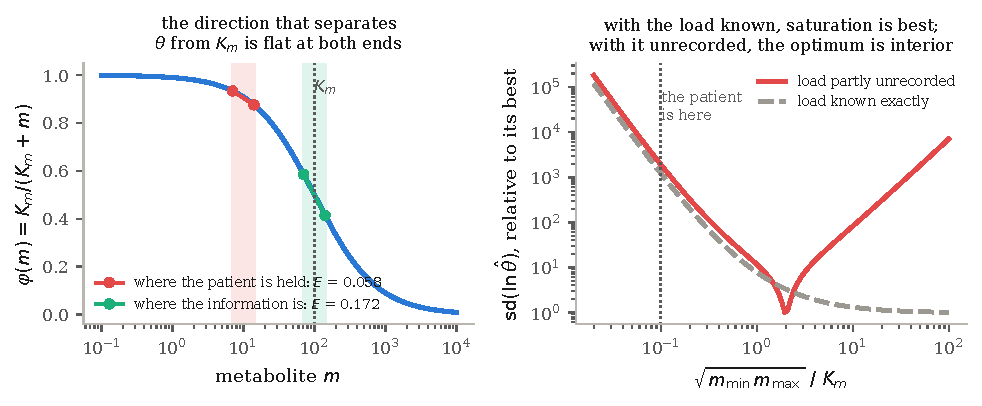
\includegraphics[width=\textwidth]{fig_D1_excitation.pdf}
\caption{The excitation condition. \textbf{Left:} $\varphi(m) = K_m/(K_m+m)$, the direction
that separates $\theta$ from $K_m$. It is flat at both ends of the saturation curve, so the
information a band carries is the \emph{drop} in $\varphi$ across it,
\eqref{eq:E}. The two shaded bands have the same fold range and differ only in where they
sit. \textbf{Right:} the price of sitting in the wrong place, as
$\operatorname{sd}(\ln\hat\theta)$ against the geometric centre of the band. With the load
known exactly the curve is monotone and saturation is the best place to measure; with the
load partly unrecorded the optimum is interior, because
Proposition~\ref{prop:excitation}(2) then bites. The dotted line is where clinical
management holds the patient.}
\label{fig:D1}
\end{figure}

\begin{remark}[Two ways to buy the same information, and only one of them is available]
\label{rem:two_buys}
Equation \eqref{eq:Emax} says a required excitation can be met either by a wide band
wherever the patient is, or by a narrow band placed correctly. The two are not
interchangeable clinically. Reaching the neighbourhood of $K_m$ means carrying the marker
to roughly twenty times its managed level, which is a decompensation; buying the same
information from the operating point instead needs a fold range of order ten, which is also
a decompensation, reached from below. \textbf{The safety constraint is on the level, and both
routes violate it.} What separates them is that the first is cheap in width and the second
is cheap in level, so a protocol that has any room at all should spend it on placement
rather than on duration.
\end{remark}

\vspace{0.5em}
\hrule
\vspace{1em}

%==========================================================================

\section{The design: where the excitation can be bought, and what it decides}
\label{sec:designsec}
%==========================================================================

\emph{Section~\ref{sec:excitation} says what a trajectory has to do. This section asks
what the accessible trajectories actually do, and what decision the answer supports.}

\subsection{What does not collapse, stays --- and what does, and why}
\label{sec:collapse}

The estimator here is the exact information filter for constant parameters,
\begin{equation}
P_k^{-1} \;=\; P_0^{-1} \;+\; \sum_{i \le k} \frac{q(m_i, \Delta_i)\,q(m_i, \Delta_i)^{\!\top}}{\sigma^2},
\label{eq:infofilter}
\end{equation}
on the augmented coordinates $(\ln\theta, \ln K_m, L_0, \ln k_e)$, none of which carries
dynamics. \textbf{There is no process noise on $\theta$, and that is a construction rather
than a setting.} A random walk on $\theta$ manufactures a finite stationary covariance in a
direction the data may never see, which is precisely the error this note exists to warn
about; with \eqref{eq:infofilter}, what does not collapse stays visibly uncollapsed.

\paragraph{The footing, stated once and used everywhere.} Four choices decide every number
in this section, and earlier drafts of this note did not hold them fixed.
\begin{enumerate}[leftmargin=*, itemsep=2pt]
\item \textbf{$q$ carries the increment}, as \eqref{eq:columns} requires. A design is
\emph{not} fully described by the levels it visits: two samples at the same level under
different $\Delta$ carry different information, and that is the whole of
Section~\ref{sec:therapychannel}.
\item \textbf{$\theta$ and $K_m$ are free.} No prior is placed on either. Stripping the
priors one at a time shows that the $K_m$ prior does no work at all --- the accessible
design gives $0.1474$ with it and $0.1474$ without it, and still $0.1474$ at a prior
twenty times looser --- so nothing here depends on knowing $K_m$, which
Remark~\ref{rem:no_km} forbids.
\item \textbf{$k_e$ carries a log-prior of $0.8$}, a factor of $2.2$, and it is the only
prior that does any work: removing it takes the same design from $0.1474$ to $0.6451$. The
gate needs $k_e$ within a factor of $2.95$, which is the one thing this note asks the
literature for.
\item \textbf{Intake varies day to day at a $10\%$ coefficient of variation, and is
recorded to $5\%$.} By Proposition~\ref{prop:rank} a perfectly steady load is the exactly
singular case, so the variability is not noise to be averaged away.
\end{enumerate}

An extended Kalman filter on the joint state was written first and is not used, for a
reason worth recording. The marker's time constant is
$\bigl((\theta+\Delta) g'(\bar m) + k_e\bigr)^{-1}$, which is $0.81$ hours at the
illustrative values, against a therapeutic increment decaying with a half-life of $3.5$
days: a separation of $104$. The marker is therefore in quasi-steady state at every
sampling instant a clinic could use and \eqref{eq:infofilter} is exact rather than
approximate. The code measures the separation rather than asserting it, and returns one
number a protocol needs: after a dose the marker is within $5\%$ of quasi-steady in $0.91$
hours and tracks to within $5\%$ thereafter, so a sample drawn inside that first hour is
not a steady state and does not belong in a steady-state fit.

\begin{figure}[htbp]
\centering
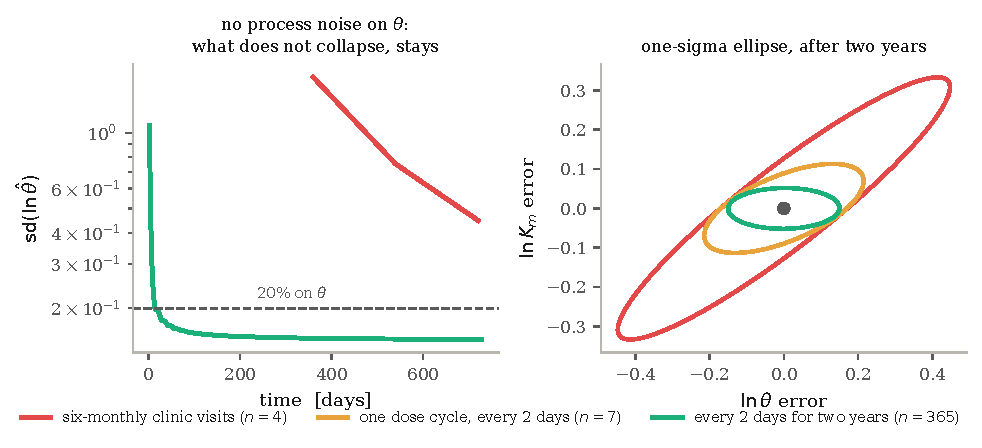
\includegraphics[width=\textwidth]{fig_D2_collapse.pdf}
\caption{Three sampling designs under the biweekly dosing schedule, over two years.
\textbf{Left:} $\operatorname{sd}(\ln\hat\theta)$ as samples arrive. \textbf{Right:} the
one-sigma ellipse in $(\ln\theta, \ln K_m)$ at the end. What separates the designs is how
much of the dose cycle they see, not how many samples they take.}
\label{fig:D2}
\end{figure}

\begin{adjustwidth}{-1.4cm}{-1.4cm}
\begin{table}[htbp]
\centering
\footnotesize
\caption{\label{tab:designs}What each design delivers. Bold is inside the $20\%$ target.
The fourth column is the range of the therapeutic increment the design actually sees, and
it, rather than $n$, is what orders the table. The last column is the same design evaluated
with the increment dropped from the sensitivity while still being used to generate the
levels, which is what earlier drafts of this note reported.}
\input{../results/tables/tab_D_designs}
\end{table}
\end{adjustwidth}

\textbf{The gate passes, and it passes on ordinary outpatient care.} Sampling monthly
across dose cycles for two years --- twenty-five draws, no excursion, no admission ---
reaches $\operatorname{sd}(\ln\hat\theta) = 0.170$, inside the $20\%$ target. Two-monthly
sampling, thirteen draws, reaches $0.187$ and also passes. Six-monthly visits reach
$0.418$ and do not.

\textbf{What separates them is not $n$.} Two-monthly sampling passes with thirteen samples
while fortnightly sampling fails with fifty-three. Read the fourth column instead: the
designs that pass are the ones that see the increment vary, and the ones that fail are the
ones that do not. Six-monthly visits catch a range of $\Delta/\theta$ of $0.45$;
two-monthly visits catch $1.94$.

\begin{remark}[Do not sample at the dose interval. This is the sharpest rule in the note.]
\label{rem:aliasing}
The fortnightly row of Table~\ref{tab:designs} is a catastrophe, and it is a
\emph{designed} catastrophe rather than bad luck. The dose interval is fourteen days, so
sampling every fourteen days lands every draw at the same phase of every cycle. The range
of $\Delta/\theta$ collapses from $1.95$ to $0.13$, the correlation between $\ln\theta$ and
$\ln K_m$ returns to $+0.998$, and $\operatorname{sd}(\ln\hat\theta)$ goes to $3.51$. The
same happens at twenty-eight days, and at any multiple.

\textbf{Moving the schedule by half a day fixes it}: sampling every $14.5$ days gives
$0.161$. A factor of twenty-two in the precision of the answer turns on a choice a protocol
writer would make for administrative convenience, and would currently make the wrong way,
because ``sample on dosing days'' is the obvious thing to write.
\end{remark}

\textbf{Three more things in that table are worth reading against what this note used to
say.}

\begin{enumerate}[leftmargin=*, itemsep=3pt]
\item \textbf{The last column is the error.} With the increment dropped from the
sensitivity, every accessible design sits between $1.0$ and $9.4$ and none of them
collapses, which is what earlier drafts reported as the result. The correction is checked
against a finite difference of the integrated dynamics in two independent ways, on two
integrators over two spans (Appendix~\ref{sec:repro}); the uncorrected column is wrong by
up to $64\%$ of itself at the top of a dose cycle.
\item \textbf{Placement still helps, and by a factor of nine rather than a hundred.} The
same $365$ samples placed to straddle $K_m$ reach $0.0157$ against $0.1499$. The straddling
design remains unavailable for the reasons of Section~\ref{sec:excursion_table}, so this is
a statement about what is being given up, not a recommendation.
\item \textbf{One dose cycle of seven samples does not do it.} It reaches $0.219$ and has a
floor there: no improvement in how well the increment is known brings it inside the target,
because what limits it is the design and not the product. An earlier report of this work
claimed that single cycle passed; it did so only with $k_e$ held known, and the claim is
withdrawn in \texttt{REVIEW\_LOG.md} rather than deleted.
\end{enumerate}

\textbf{And the load record behaves in the way Proposition~\ref{prop:rank} says, not the
way this note used to assume.} Recording the load ten times better --- to $0.5\%$, which
nobody can do --- moves the dense design by about one per cent. That retires the claim that
load-record \emph{precision} is the binding design variable. What the record has to contain
instead is \emph{variation}: by Proposition~\ref{prop:rank} a perfectly steady intake is the
exactly singular case, and half a per cent of day-to-day variability restores full rank.

\begin{remark}[What the filter claims, and what a prior-free fit says instead]
\label{rem:priorfree}
Table~\ref{tab:designs} reports posterior standard deviations under one prior, and that
prior is load-bearing. With \emph{no} prior at all --- $k_e$ free as well --- the same
two-daily design gives $\operatorname{sd}(\ln\hat\theta) = 1.03$, and a prior-free
nonlinear least squares started half a decade from the truth does worse still, because
along the near-null direction of Proposition~\ref{prop:rank} the gradient is third order
and a started-away optimiser does not climb back. \textbf{So the honest claim is
conditional and is stated as such: this design identifies $\theta$ to better than $20\%$
\emph{given} $k_e$ within a factor of about three, and does not identify it at all
without.} What survives unconditionally is the comparison --- carrying the increment is
worth between one and two orders of magnitude on every design in the table, prior-free ---
and it is the comparison, not the absolute number, that the data specification rests on.
\end{remark}

\subsection{Where the excitation could come from}
\label{sec:excursion_table}

Each accessible source of variation moves the marker by a known amount, in a known
direction, from a known place. Table~\ref{tab:excursion} evaluates \eqref{eq:E} on each.

\begin{adjustwidth}{-1.0cm}{-1.0cm}
\begin{table}[htbp]
\centering
\footnotesize
\caption{\label{tab:excursion}Excitation available from each source, against the
$E \approx 0.50$ the decision requires. Direction matters: the curvature is at high $m$, and
most of what a chart contains moves the patient the other way. The last column is how much
of the excitation a band of that fold range \emph{could} have delivered if it had straddled
$K_m$, so it separates being too narrow from being in the wrong place.}
\input{../results/tables/tab_D_excursion}
\end{table}
\end{adjustwidth}

Three readings.

\begin{enumerate}[leftmargin=*, itemsep=3pt]
\item \textbf{Everything routine is in the wrong place, not merely too narrow.} The
inter-dose recovery, the carnitine dose steps and the cyclical antibiotics all deliver
between a fifth and a quarter of what their own fold range could deliver, because they
happen an order of magnitude below $K_m$. Widening them does not fix that.
\item \textbf{Only a decompensation gets close, and it is still short.} An excursion from
the operating point to eight times it reaches $E = 0.35$ against the $0.50$ required, and it
does so at $74\%$ of what that fold range could deliver, because it at least moves towards
$K_m$. \textbf{The excitation the decision needs is available only from the event the
treatment exists to prevent}, and even then not in full.
\item \textbf{A labelled-propionate bolus is the one designed source, and it is small.}
Doubling the marker from the operating point reaches $E = 0.076$. Its value is not the
excitation it supplies but that it measures capacity on a different axis entirely, which is
the subject of Section~\ref{sec:validation}.
\end{enumerate}

\subsection{The estimand is a decision, and the decision survives what the parameter does not}
\label{sec:decision}

Confidence intervals on $\theta$ are the wrong output. The clinical question is the
\emph{sign} of $\mu = \theta - \thc$, and its two errors are not interchangeable: treating a
patient who does not need it costs an infusion and a venous line, and failing to treat one
who does costs a decompensation. Figure~\ref{fig:D3} is the operating characteristic of that
decision.

\begin{figure}[htbp]
\centering
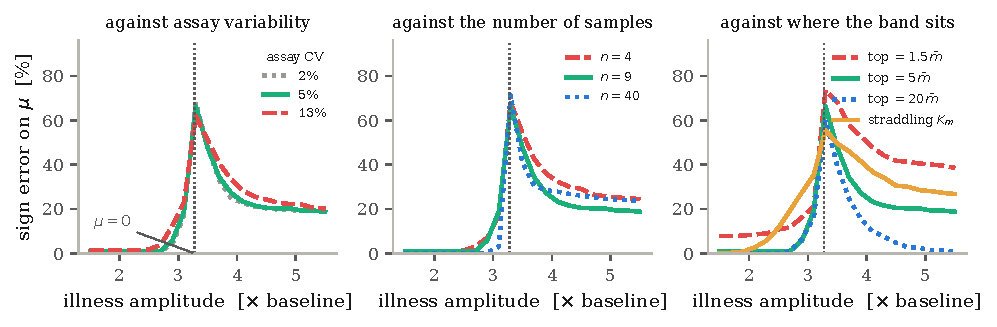
\includegraphics[width=\textwidth]{fig_D3_decision.pdf}
\caption{The probability of getting the sign of $\mu$ wrong, by simulation, as a patient of
fixed biology is swept across the decision boundary by the illness amplitude. Left of the
dotted line the error is a patient treated who did not need it; right of it, a patient left
untreated who did. Each panel varies one thing a protocol controls.}
\label{fig:D3}
\end{figure}

\begin{center}
\footnotesize
\begin{tabular}{@{}rrlrr@{}}
\toprule
\textbf{illness} & $\mu$ & \textbf{which error} & \textbf{simulated} &
\textbf{a delta method would say} \\
\midrule
$1.50\times$ & $+2006$ & treat unneeded & $0.2\%$  & $39.5\%$ \\
$2.50\times$ & $+876$  & treat unneeded & $0.2\%$  & $38.8\%$ \\
$2.98\times$ & $+339$  & treat unneeded & $6.0\%$  & $36.1\%$ \\
\addlinespace
$3.58\times$ & $-339$  & fail to treat  & $\mathbf{52.5\%}$ & $42.3\%$ \\
$4.00\times$ & $-818$  & fail to treat  & $31.8\%$ & $41.1\%$ \\
$5.50\times$ & $-2513$ & fail to treat  & $26.0\%$ & $40.4\%$ \\
\bottomrule
\end{tabular}
\end{center}

\textbf{The two errors are not the same size, and the larger one is the one that costs a
patient a decompensation.} At equal distance from the boundary --- $|\mu| = 339$ on either
side --- the simulated error is $6\%$ for treating a patient who did not need it and $53\%$
for failing to treat one who did. The asymmetry does not close with distance: at
$|\mu| = 2513$ on the unsafe side the error is still $26\%$, where at $|\mu| = 2006$ on the
safe side it is $0.2\%$. \textbf{The estimator fails towards declaring patients safe.} The
mechanism is already in this note: by Remark~\ref{rem:eiv} the abscissa noise inflates
$\hat a$ and hence $\hat\theta$, and $\hat\mu = \hat\theta - \thc$ inherits that bias
whole.

The simulated error exceeds $10\%$ for every illness amplitude from $3.10\times$ baseline
upward, which is the whole region at and beyond the decision boundary at $3.28\times$. A
protocol reporting this design's answer would be reporting a test that is nearly reliable
where it does not matter and close to a coin toss where it does.

\textbf{What excursion would fix it, and whether one exists.} Asking the same question of a
patient $30\%$ below the threshold, the simulated sign error falls from $36\%$ at a
two-fold excursion to $10\%$ at twenty-fold and then \emph{plateaus near $6\%$}: past about
forty-fold, more excursion buys nothing. The plateau is the load-bias degeneracy of
Proposition~\ref{prop:excitation}(2), which excursion does not touch. So there is no
excursion, survivable or otherwise, that delivers a $5\%$ sign error at this load record ---
and the requirement that does bite, a twenty-fold excursion for a one-in-ten error, is a
severe decompensation. Table~\ref{tab:spec} carries the whole curve.

\begin{remark}[Why this is simulated and not propagated]
\label{rem:no_delta}
A delta-method calculation, propagating the estimator's covariance to $\mu$ and reporting
$\Phi(-|\mu|/\operatorname{sd}(\hat\mu))$, is available and is wrong here, in a way that
matters. At the accessible design $\operatorname{sd}(\hat\mu)/|\mu| = 3.7$, so a Gaussian
of that width crosses zero about $39\%$ of the time. Simulating the same model instead,
$\hat\theta$ ranges over three orders of magnitude across replicates --- the design really
is that bad --- and $\hat\mu$ never changes sign.

The two disagree because $\hat\mu$ is not symmetric about $\mu$. The design's near-null
direction is very nearly the direction along which $\mu$ is monotone and of one sign, so the
sampling distribution of $\hat\mu$ is heavily skewed and does not cross zero anything like
as often as its standard deviation suggests. \textbf{That is the margin theorem of
\eqref{eq:mufibre} showing up in the estimator}, and taking the Gaussian tail at face value
would throw away the one favourable result this note has. Both numbers are reported by the
code so that the gap stays visible.
\end{remark}

\vspace{0.5em}
\hrule
\vspace{1em}

%==========================================================================

\clearpage
\section{The data specification}
\label{sec:spec}
%==========================================================================

\emph{Every row is generated from the model code and is a consequence of something proved
above. It has two tiers, and the order is not cosmetic: Tier~1 is a single measurement
nobody has published, and until it reports there is no defensible answer to the question
Tier~2 asks.}

\begin{adjustwidth}{-1.4cm}{-1.4cm}
\begin{table}[htbp]
\centering
\footnotesize
\caption{\label{tab:spec}What a record would have to contain for $\theta$ to be
identifiable. Quantities are in observable units, not multiples of $K_m$, because $K_m$ is
not known --- and by the last row does not need to be.}
\input{../results/tables/tab_D_spec}
\end{table}
\end{adjustwidth}

\subsection{Tier 1: the measurement the method's feasibility turns on}
\label{sec:tier1}

\textbf{What to run.} One cohort, two $1$-$^{13}$C-propionate breath tests bracketing a
single dose, on one day. The quantity measured is the repeatability of the assay
\emph{within a day and within a state}, which is what a pre/post pair around a dose depends
on.

\textbf{Why it is first.} By Section~\ref{sec:excitation} the therapy channel is what makes
$\theta$ identifiable, and \eqref{eq:dosereq} is stated in units of $\theta$: the ratio
$\Delta/\theta$ is only as well known as $\Delta$ is. Section~\ref{sec:designsec} turns
that into one number --- the delivered increment must be characterised to about $12\%$ for
monthly sampling to reach the $20\%$ target on $\theta$. \textbf{Everything the therapy
channel buys is conditional on that, and it has never been measured.}

\textbf{What is published is an upper bound, and it is not the quantity needed.} The only
repeatability data for this assay~\cite{breath_test_mma} % C48
are between-visit: controls repeated at one- to three-week intervals, and fifteen
\emph{mut} patients at separate visits \emph{two months to four years apart}, with the
authors naming changing renal status and varying $V\mathrm{CO}_2$ as causes. The Results
give $14.02 \pm 12.86\%$ with a range of $0.39$ to $50.84\%$; the abstract's widely quoted
$12.8\%$ is the standard deviation of the per-subject coefficients, not their mean. And the
cohort is methylmalonic acidemia, not propionic acidemia, where the block sits at PCC
itself.

Between-visit variation is an \emph{upper bound} on same-day error, because it contains
drift a same-day pair removes, and the bound sits close to the requirement. \textbf{But a
bound that happens to sit near a threshold is not a measurement of it}, and a per-subject
range reaching $50.8\%$ cannot be applied to an individual. Tier~1 replaces an inference
with a number.

\subsection{Tier 2: conditional on Tier 1, and then it is a small study}

\paragraph{Cover the dose cycle; do not chase the marker.} Monthly draws across dose cycles
for two years reach the target, and two-monthly draws --- thirteen over two years --- also
reach it. This is ordinary outpatient blood work. What buys the information is the
\emph{phase}, not the rate: a schedule that sees the increment vary identifies $\theta$ and
one that does not, does not, whatever its density.

\paragraph{And one hard exclusion a protocol would currently get wrong.}
\textbf{Do not sample on dosing days, or at any multiple of the dose interval}
(Remark~\ref{rem:aliasing}). ``Draw bloods when the patient attends for dosing'' is the
natural thing to write and it is the one schedule that destroys the result: every draw
lands at the same phase, the range of $\Delta/\theta$ collapses from $1.95$ to $0.13$, and
$\operatorname{sd}(\ln\hat\theta)$ goes from $0.17$ to $3.51$. Moving the schedule half a
day recovers it.

\paragraph{The load record: ordinary precision, and keep the variation.} Recording intake
twenty times more precisely buys about six per cent, so precision is not the binding
variable. The variability is subtler and enters twice. By Proposition~\ref{prop:rank} a
perfectly steady load makes the design exactly rank deficient, and that null direction must
be filled by something; as the specification stands it is filled by the $5\%$ prior on the
load bias, and only real day-to-day variation lets the \emph{data} fill it instead. So
``record intake as eaten, do not smooth it'' is the difference between a result the data
support and one a prior supports. It costs nothing: it is an instruction to omit a
data-cleaning step, not to add a measurement.

\paragraph{$k_e$, and nothing else, is assumed.} The result needs the non-enzymatic
clearance within a factor of about three, which the literature supplies; no measurement
programme is proposed for it. $K_m$ is assumed at nothing: a prior twenty times looser
leaves every number unchanged, which is what Remark~\ref{rem:no_km} demanded.

\subsection{What is excluded, and what is not promised}

Two acquisitions an earlier draft asked for are struck out. \textbf{High-frequency sampling
at a fixed operating point} buys nothing: two-monthly sampling with thirteen draws beats
fortnightly sampling with fifty-three, because the first sees the dose cycle and the second
is aliased against it. \textbf{Decompensation records} are excluded twice over --- the
excursion is not observed at the magnitude required, and by Section~\ref{sec:discussion}
the model does not hold in that regime.

\textbf{And the specification does not promise a decision.} It buys an identified $\theta$.
Section~\ref{sec:decision} shows that the sign of the margin does not follow from it, for
reasons that are not about the data, and Section~\ref{sec:scope} shows that $\theta$ itself
stops being recoverable in the patients the question matters most for. A protocol written
from this page should report $\hat\theta$ with its interval and should not be read as a
rule for escalating an individual patient.

\vspace{0.5em}
\hrule
\vspace{1em}

%==========================================================================

\section{Limits of recoverability}
\label{sec:scope}
%==========================================================================

\emph{This section is a scope limit on everything above, stated here rather than in a limitations paragraph because it bites hardest in the population the question matters
most for.}

In \eqref{eq:local} the alternative channel does not saturate, so as residual capacity
falls the marker does not rise without bound. It approaches a ceiling set by that channel
alone,
\begin{equation}
m \;\longrightarrow\; \frac{L_0 + L}{k_e} \qquad \text{as } \theta \to 0,
\label{eq:ceilinglimit}
\end{equation}
which at the illustrative values is $6.45$ times the managed level. The elasticity of the
marker to capacity dies with it.

\begin{center}
\footnotesize
\begin{tabular}{@{}rrr@{}}
\toprule
$\theta$, as \% of nominal & marker, $\times$ managed & $\lvert\partial \ln m / \partial \ln\theta\rvert$ \\
\midrule
$100\%$ & $1.00$ & $0.915$ \\
$50\%$  & $1.82$ & $0.807$ \\
$20\%$  & $3.41$ & $0.537$ \\
$10\%$  & $4.57$ & $0.321$ \\
$5\%$   & $5.40$ & $0.173$ \\
$2\%$   & $6.00$ & $0.072$ \\
$1\%$   & $6.22$ & $0.036$ \\
\bottomrule
\end{tabular}
\end{center}

Stated in the units a clinic reads: once a patient's managed marker sits above
about three to four times the reference level, residual capacity is no longer recoverable
from it. The elasticity falls below $0.5$ at $3.6$ times managed, below $0.25$ at $5.0$,
and below $0.1$ at $5.8$. At the bottom of that table two patients differing tenfold in
capacity, $10\%$ of nominal against $1\%$, are separated by less than a third in
marker level, which no assay resolves against the day-to-day variability of the quantity.

\subsection{What the estimate's own precision does across that range}
\label{sec:scopeprec}

The table above is about the \emph{marker}. The same question can be put to the
\emph{estimate}, and until now it had not been: every precision this paper reports is
computed at $\theta = 3000$, and on the table above that is the $100\%$ row.

That is worth stating plainly, because the repository had left it ambiguous.
\texttt{src/common/models.py} annotates $\theta = 3000$ as $V_{\max}$, the \emph{maximal}
enzymatic velocity, and annotates the parent model's $\theta = 300$ as ``$\sim 10\%$ of
normal''. Together those put normal at $3000$ and the local block at $100\%$ of it, so the
local block is a normal-capacity illustration and Table~\ref{tab:params} now labels it as
one. Residual PCC activity in propionic acidemia is under $5\%$ of
control~\cite{pcc_residual_activity}, so the patient sits at $\theta \le 150$, which the
table now carries as its own row. Nothing about the model changes; what changes is that the
illustration is no longer available to be read as a description of the patient.

Holding the recorded load fixed and letting the marker rise, which is the convention the
table above already uses, and re-solving the operating level, $\sigma$, the load-bias prior
and the excitation at each capacity:

\begin{center}
\footnotesize
\begin{tabular}{@{}rrrrr@{}}
\toprule
$\theta$, as \% of nominal & marker, $\times$ managed &
$\lvert\partial \ln m / \partial \ln\theta\rvert$ &
$\operatorname{sd}(\ln\hat\theta)$ & monthly visits to $0.20$ \\
\midrule
$100\%$ & $1.00$ & $0.915$ & $\mathbf{0.1699}$ & $11$ \\
$20\%$  & $3.41$ & $0.537$ & $0.8107$ & --- \\
$10\%$  & $4.57$ & $0.321$ & $1.5830$ & --- \\
$5\%$   & $5.40$ & $0.173$ & $3.0673$ & --- \\
$2\%$   & $6.00$ & $0.072$ & $7.4572$ & --- \\
\bottomrule
\end{tabular}
\end{center}

\noindent
Medians over $24$ simulated intake records at the specification's own $10\%$ day-to-day
variability; the seed ranges are in \texttt{audit/n4\_theta\_scope.py}. A dash means the
target is not reached at any number of monthly visits up to $600$, which is fifty years of
follow-up.

$\operatorname{sd}(\ln\hat\theta)$ is not monotone in $\theta$, so the gate is crossed twice.
It holds for $\theta$ between $2472$ and $18814$, which is $82\%$ to $627\%$ of nominal, a
band of $7.6$ fold, with the best precision $0.123$ at about twice nominal. Below the band
the marker has stopped responding to capacity, which is the statement above. Above it the
$\theta$ column saturates at $L$ while the assay term keeps growing, so information per draw
stops improving. \textbf{The disease sits a factor of $16$ below the lower edge of the band
the design works in.} Sampling every two days for two years instead of monthly, fifteen times
the draws, moves that edge only from $82\%$ to $75\%$ of nominal. That $9\%$ is the
quantitative form of the sentence below: it is not a statement about sampling effort.

One consequence follows for the dose and it is independent of the precision. The
admissibility bound $\theta + \Delta_{\mathrm{peak}} \le$ normal is satisfied at the
illustrative point only because the check reads $\theta$ as the \emph{residual} and infers
normal as $\theta/0.05$; written out, its verdict is
$\operatorname{frac} \times (1 + \Delta_{\mathrm{peak}}/\theta)$ with $\theta$ cancelled,
which cannot report a breach below a residual activity of $32\%$ and so cannot bind on this
disease at all. Read instead with $\theta = 3000$ as normal and $D$ held at its booked value
rather than scaled with capacity, which is what a dose in mg/kg is, the bound is breached at
$10\%$ of nominal and below: at $5\%$ the booked increment would drive the enzyme to $2.18$
times normal, and the largest admissible increment there is $D = 2672$ rather than $6000$.
That does not rescue the precision, since at $D = 2672$ and $\theta = 150$ the monthly design
returns $2.96$, but it is a second and independent reason to think the increment is set too
high, alongside the trial's own reported falls in the $D$ row of Table~\ref{tab:params}.

This is the severely affected patient. The population in which the dosing question
is most urgent is the population in which the record cannot answer it. This is not a statement about sampling effort: no schedule, no excursion and no precision on the dose
recovers a quantity the observable has stopped responding to. The therapy channel of
Section~\ref{sec:excitation} does not rescue it either: it supplies excitation in
$\theta$ against $K_m$, not sensitivity of $m$ to $\theta$.

One consequence is favourable and should not be lost in the statement of a
limit. What dies here is the estimate of \emph{capacity}. A prediction read directly off
the marker does not die, because the marker is what is measured. So the failure is
asymmetric: it falls on the mechanistic quantity and not on the observable, which is an
argument for keeping claims close to the observable in exactly this population.

\vspace{0.5em}
\hrule
\vspace{1em}

%==========================================================================

\section{Discussion}
\label{sec:discussion}
%==========================================================================

Everything above sits inside two boundaries. These are claims about identifiability, a
property of a model and a design together, not about patients: every design number is
computed from \eqref{eq:local} with the constants of Table~\ref{tab:params}, of which
three are taken from the literature and the rest are assumed, so what the analysis establishes is
what a record \emph{of the kind assumed} could yield \emph{under the model assumed}.
Whether a real record behaves that way turns on the observation model of
Remark~\ref{sec:marker}, that a marker which is not the enzyme's substrate tracks it
monotonically, and that assumption is not testable from anything published.

The second boundary is that the model questions its own validity in the regime the
excursion argument points at --- and the boundary is narrower and better located than
``the model may not hold out there''.

\emph{Every multiple in this paragraph is a multiple of the parent's own reference level,
which is not the local model's.} The parent \eqref{eq:parent} sits at an attractor of
$\num{parent_mbar}$ at its own capacity and load, where the local model's managed level
is $\bar m = 10$; the two are different quantities and a ratio taken against one does not
transfer to the other. Read against $\num{parent_mbar}$, the parent has a clearance
maximum at $\num{peak_over_mbar}$ times it and a separatrix at $\num{sep_over_mbar}$ times
it at baseline load. The \emph{stable equilibrium is lost at the first of those, not the
second}: raising the load walks attractor and separatrix together until they collide at
the fold of \S\ref{sec:model}, and they merge at $m = \num{fold_m}$, which is the
clearance maximum, at a load of $\num{fold_load}$, or $\num{fold_load_ratio}$ times
baseline. The separatrix at $\num{sep_over_mbar}$ times the attractor is how large a
perturbation must be to escape the basin at baseline load, which is a different and also
useful number.

Both estimators here are steady-state fits, and $\num{band_beyond_pct}\%$ of a band
running to eight times the parent's reference level, $\num{band_parent}$, lies beyond that
clearance maximum, where the parent says there is no steady state to fit. Fitting the
local model to the parent's own noiseless clearance over that band recovers
$\hat\theta = \num{fit_theta_hat}$ for a patient whose true capacity is the parent
model's $\theta = 300$, against an intrinsic threshold of $\num{theta_crit}$: so
misspecification alone, with no noise and no perturbation, eats
$\num{fit_margin_eaten_pct}\%$ of a true margin of $+\num{fit_margin_true}$ and leaves
$+\num{fit_margin_est}$.

\emph{That fit has to be specified, because the number moves with its definition.} The
levels are $\num{fit_levels}$, spaced geometrically from the parent's reference level to
$\num{fit_band_top}$ times it; the load at each is the parent's own noiseless clearance
there; and what is fitted is the \emph{balance} this paper's estimator actually solves,
$s = \theta\,g(m,K_m) + k_e m + b$ with $K_m$ at its population value, $\theta$ and $k_e$
non-negative and the load constant $b$ \emph{free}, by unweighted least squares in the
load. The free $b$ is the part that matters: the estimator of \S\ref{sec:collapse}
carries a load constant it does not know, and a fit of one clearance curve onto another
does not, which makes the curve-to-curve reading a different and much more favourable
exercise.

\textbf{The fit lands on the boundary of admissibility, and that, rather than the number
it lands at, is the finding.} On every band $\hat k_e$ sits exactly on its lower bound of
zero. Released, it goes \emph{negative} --- $\num{fit_ke_hat_free}$ at this band --- and
$\hat\theta$ rises to $\num{fit_theta_hat_free_ke}$. So the local form's best
approximation to the parent's clearance here describes a patient who clears the metabolite
by a route running backwards, and the best \emph{admissible} approximation describes one
with no non-enzymatic clearance at all. Neither is a patient. \emph{Over this band the
local family represents the parent only at its own edge.}

Two things follow, and the first disarms the number. \textbf{A boundary solution is not a
point estimate}: $\hat\theta = \num{fit_theta_hat}$ is where the constraint stops the fit,
not where the likelihood peaks, so the gap between it and
$\theta_{\mathrm{crit}} = \num{theta_crit}$ is not a margin and should not be read as
one --- a conclusion that holds whatever the spacing and the weighting, and therefore more
firmly than the spread below. \textbf{And nothing in the fit would reveal any of it.} The
admissible fit's residual over these levels is $\num{fit_resid_sigma}$ of a single $5\%$
error in the recorded load, which is the accuracy
Section~\ref{sec:tierload} asks for: the misspecification is invisible in exactly the
diagnostic that would be used to look for it, which is the same \emph{symptom}
Section~\ref{sec:structuredep} finds for the published alternative by a different
mechanism --- \S\ref{sec:pattern2} takes the two together.

\emph{What is robust here is that the margin is consumed, not what is left of it.} Three
equally defensible readings move $\hat\theta$ at the same band: weighting the residual by
the load, which is what a multiplicative load error implies, gives
$\num{fit_theta_hat_rel}$; reading ``over the band'' as a dense grid rather than the
design's own nine levels gives $\num{fit_theta_hat_dense}$; spacing the nine levels
linearly gives $\num{fit_theta_hat_lin}$. Against
$\theta_{\mathrm{crit}} = \num{theta_crit}$ those span an estimated margin from about
$-4$ to $+9$, so \textbf{the sign of what survives is not determined by the data at all},
and the $+\num{fit_margin_est}$ above is the design's own nine levels and nothing more
general. The conclusion that carries is the one that holds across every reading: a
noiseless, unperturbed fit of the admissible local form to the parent over this band
consumes essentially the whole of a $+\num{fit_margin_true}$ margin. And the two models
disagree by a factor of $\num{clear_ratio}$ about the largest load a patient can clear:
the local model needs $\num{hold8_ratio}$ times baseline to hold eight times \emph{its}
managed level, $\num{band_local}$, while the parent cannot clear more than
$\num{fold_load_ratio}$ times baseline at all.

\textbf{What the boundary does \emph{not} reach is the design's own operating points, and
that is a bound rather than a hope.} The local model's marker obeys
$\dot m \le L - k_e m$, so every trajectory at the recorded load is capped at
$L/k_e = \num{local_ceiling}$; and the parent's clearance maximum cannot fall below
$\sqrt{K_c M_i} = \num{peak_floor}$ at any capacity, because that is where the alternative
route's own derivative turns. A margin of $\num{peak_margin}$, so \emph{no} operating
point of any design in this paper lies past the parent's clearance peak, at any capacity
in Table~\ref{tab:scope}. Only the excursion band --- which the paper declines to use ---
goes beyond it. That margin is a property of the constants carried here and not a theorem:
across this paper's own prior range for $K_c$, $M_i$ and $\rho_0$, fewer than
$\num{prior_floor_pct}\%$ of parameter draws even place $\sqrt{K_c M_i}$ below
$L/k_e$, and fewer still actually reverse it.

The decompensation route is therefore excluded three times over: the excursion it would
supply is not observed at the magnitude required, the model that would interpret it does
not hold there, and the reduction through which that model is evaluated is not reliable
there either.

The third reason has the same shape as the first two, and it is the one this paper acquired
last. Everything computed from \eqref{eq:alphaqss} anywhere above is computed at a fixed
point, and at a fixed point the reduction is exact as an identity rather than as an
approximation (Section~\ref{sec:reduction}). A decompensation is precisely the regime in
which the quantity of interest is a trajectory and not a fixed point, and there the two
formulations part company: the reduced and two-state systems differ by $3.4\%$ to $25.4\%$
along the approach to equilibrium, and the basin boundary itself sits up to $49.6\%$ away
from the reduced separatrix when carnitine starts at its pre-perturbation value, which is
what a sudden load spike leaves behind. The displacement is signed and the unsafe sign is
the reachable one: from a depleted pool the boundary falls \emph{below} the reduced
separatrix, so there the closed form calls safe a state the parent escapes from. So the one
regime that would supply the excursion is also the one regime in which the closed form
carries no warrant. The route is not narrowly missed; it is excluded on the excursion, on
the model, and on the reduction, independently.

\subsection{What the five results amount to}

\textbf{The contribution is the design rules, with a scope condition attached, and not the
capacity estimate.} What transfers is a set of statements about identifying a saturable
channel from a marker under a known periodic input: carry the input as a regressor, never
sample at its period or a multiple of it, record the driving load as eaten and to a stated
accuracy, and establish where in the parameter range the target is recoverable before
quoting a precision anywhere in it.

The first result is actionable now and survives the scope limit: the excitation is already
being administered, and a protocol loses a factor of $\num{alias_cost}$ against monthly draws by scheduling bloods
on dosing days, which is still a factor of $16$ at a disease-range capacity where the estimate itself
is gone. The second should change how the problem is posed. Near normal capacity the
decision is blocked not by identifiability but by its own boundary, which is stipulated
rather than measured and which no better estimate of $\theta$ and no larger cohort can
repair; in the disease range both block. The third and fourth bound what should replace it, and the fifth says what the whole of it
is relative to.
The only endpoint evidence reports a smooth dose--response and no threshold, which argues
against the dichotomy rather than for a better-placed one, and an expected event rate does
not serve either: at the operating point the model-based rate is thirteen times
\emph{worse} than reading the same rate off the measured marker, the published exponent is
known only to a factor of $4.8$, and the map has no published reference concentration to
anchor it.

What is left where capacity is not recoverable is not nothing: $K_m$ is determined at every
capacity, the record still supplies an upper bound on $\theta$, and every design rule
holds. What is gone is the point estimate, and that argues for an external measurement
rather than a larger study.

\subsection{A common pattern across three of them}

Three degeneracies appear in this paper, reached by unrelated routes and concerning
different parameters. They have the same shape, and naming it is the most portable thing
here. The excitation is a product of a therapy factor and a marker factor,
$-(1 + \Delta(t)/\theta)\,\varphi(m)$, of which the literature had measured only the
second, so what the dose train contributes is not a bigger increment but a \emph{moving}
one. Proposition~\ref{prop:rank} is exactly singular at a constant recorded load and names
its own cure, so what closes it is the day-to-day \emph{variability} of ordinary eating,
while the record's \emph{accuracy} is a separate requirement entering through $\sigma$. And
the channel-exchange result (supplement, \S S1.11.1) breaks an exchange only when the inputs on
two channels differ \emph{non-constantly}, a constant increment being absorbed into the
amplitude it rides on however large it is.

In every case the separating quantity is a difference that moves, and in every case the
intuitive alternative fails: a bigger increment does not substitute for a varying one, nor
a more precise load record, nor a larger constant input. \emph{Magnitude, precision and
presence are each the wrong axis, and each is the axis a study would naturally be designed
to improve.} Two of the three are worse than neutral. A dietary record \emph{tightened} by
averaging to a weekly mean is more precise and destroys the variability
Proposition~\ref{prop:rank} needs, so Section~\ref{sec:spec} asks for a data-cleaning step
to be omitted rather than a measurement added; a \emph{steadier} administration route
removes the therapy's excitation entirely (Section~\ref{sec:route}). A larger dose is the
exception, since it raises $\Delta/\theta$ and does help, which is worth saying because it
is the only one of the three obvious moves that does.

This is a pattern across three results and not a theorem: they are three calculations that
happen to resolve the same way, and nothing here says they must. What can be said is
narrower and still useful. In a saturating compartment model observed through one marker, a
design's information sits in what varies across its samples rather than in the levels the
samples sit at, and a reader carrying that to another system should check the three
separately rather than assume the shape transfers.

\subsection{A second pattern, across the two misspecification results}
\label{sec:pattern2}

Two results here are about a \emph{wrong structure} rather than a degenerate one, and they
were reached by routes with nothing in common. Section~\ref{sec:structuredep} fits
\eqref{eq:local} to records generated by a published alternative readout and recovers a
capacity too \emph{high}, by a factor of $1.3$ to $2.0$ at this paper's own dose. The
opening of this section fits the same form to the parent's own noiseless clearance across
the excursion band and recovers one too \emph{low}, $\num{fit_theta_hat}$ against a true
$300$. The mechanisms are unrelated: the first is a free marker offset carried alongside a
free amplitude, the second a curved alternative channel that a linear $k_e m$ cannot
follow, which drives $\hat k_e$ onto its bound.

What they share is the symptom, and that is the portable part. \textbf{In both, the fit's
residual stays inside the noise the specification already asks for} --- under a fifth of
one $\sigma$ in the first, $\num{fit_resid_sigma}$ of a single load error in the second
--- \textbf{while the capacity it returns is wrong.} So on this model \emph{residual size
does not bound structural error}: the diagnostic a reader would naturally reach for to
detect a wrong structure is the one diagnostic that cannot see it. That is why
Section~\ref{sec:tierstruct}'s single blood draw is a \emph{structure} test and not a
goodness-of-fit threshold --- it separates the two structures where they disagree, in the
minutes after an infusion, instead of asking how well either fits.

And the two err in \emph{opposite} directions, which forecloses the obvious repair. A bias
of known sign could be carried as a correction or as a one-sided bound; these cannot,
because nothing in a record says which structure is the wrong one. As above this is a
pattern across two results and not a theorem. What can be said is narrower and still
useful: a small residual is evidence about noise and not about structure, and a study that
means to establish a structure has to do it with a designed discriminant rather than with a
fit.

\subsection{What would change the answer}

A same-day paired repeatability figure for the breath test, which does not exist and which
Tier~2 of Section~\ref{sec:spec} asks for, since everything the therapy channel buys is
conditional on the delivered increment being characterisable. An endpoint model that does
not require a threshold, built on the natural history study's own hazard formulation, which
needs the reference concentration and the model specification that publication does not
report. A marker that is the substrate, or an assay of it, which would remove the
observation-model assumption the whole construction rests on and is the single change that
would most enlarge what a record can support. And an external anchor on $\theta$: capacity
is identified relative to the model structure, and Section~\ref{sec:structuredep} exhibits
a published alternative under which it is not identifiable at all, fitted at a residual too
small to notice, while Section~\ref{sec:scopeprec} reaches the same place from the flux
identity and adds that in
the disease range the record does not bound $\theta$ from below whatever the structure.
Tier~2 is the only anchor here outside the longitudinal record, and a second one
independent of it would turn every statement about the value of $\theta$ from conditional
into checkable.

\vspace{0.5em}
\hrule
\vspace{1em}

%==========================================================================


\clearpage

\section*{Code and data availability}
Every figure, table and quoted number in this paper is produced by the code that
accompanies it, and the repository is the provenance for all of them: each table
is written by the function that computes it, each quantity the text quotes is
written to a generated file the text reads, and a check regenerates them and
fails the build if a committed artefact no longer matches its generator. No
patient data were used. The clinical record this paper specifies does not exist
yet; every record analysed here is simulated from the model of
Section~\ref{sec:model} with the constants of Table~\ref{tab:params}, and the
seeds are fixed and named so that every number reproduces.

\section*{Funding}
[funding statement]

\section*{Acknowledgements}
[acknowledgements]

\section*{Conflicts of interest}
[conflicts of interest]

\clearpage
\printbibliography[title={References}]

\end{document}
"
% The default build omits it.
\documentclass[11pt,a4paper]{article}

% `draft` is article's own option, and it is detected here by its effect
% rather than by reading the option list, so that it is seen whether it is
% written into \documentclass above or handed over with \PassOptionsToClass
% on the command line. article's draft mode sets \overfullrule; nothing else
% in this preamble does.
\makeatletter
\newif\ifshowregister
\ifdim\overfullrule>\z@ \showregistertrue \fi
\makeatother

% Both of article's draft-mode effects are now undone, so the register build
% is otherwise identical to the default one: no rules in the margin, and no
% blanked figures. graphicx is pulled in by tikz, so its option has to be
% passed rather than given at load time, and passed before any package loads.
\overfullrule=0pt
\PassOptionsToPackage{final}{graphicx}

\usepackage[T1]{fontenc}
\usepackage[utf8]{inputenc}
%\usepackage{lmodern}
\usepackage[margin=2.1cm]{geometry}
\usepackage{changepage}
\usepackage{amsmath,amssymb,amsthm}
\usepackage{booktabs}
\usepackage{longtable}
\usepackage{array}
\usepackage{tikz}
\usetikzlibrary{arrows.meta,positioning,shapes.geometric,calc}
\usepackage{graphicx}
\graphicspath{{../results/figures/}{results/figures/}}
\usepackage{caption}
\usepackage[colorlinks=true,linkcolor=black,citecolor=black,urlcolor=blue]{hyperref}

% Bibliography. refs.bib is GENERATED by tools/fetch_refs.py from
% paper/refs.sources; do not edit it.
\usepackage[backend=biber, style=numeric-comp, sorting=none,
            maxbibnames=6, minbibnames=3, giveninits=true]{biblatex}
\addbibresource{refs.bib}
\usepackage{enumitem}
\usepackage{xcolor}

\definecolor{accent}{RGB}{122,47,47}
\definecolor{soft}{RGB}{244,242,238}

\newtheorem{assumption}{Assumption}
\newtheorem{remark}{Remark}
\newtheorem{proposition}{Proposition}

\newcommand{\thc}{\theta_{\mathrm{crit}}}
\newcommand{\spk}{s_{\mathrm{peak}}}



\title{\textbf{The Dose Train is the Identification Experiment:\\
Estimating Residual Enzymatic Capacity in Propionic Acidemia}}
\author{Guido Putignano\\[2pt]
  \normalsize\itshape \textnormal{[affiliation]}\\
  \normalsize\texttt{[corresponding author e-mail]}}
\date{\today}

\begin{document}
\maketitle

\begin{abstract}
\noindent
The clinical decision in mRNA enzyme replacement for propionic acidemia is a dosing
interval. It is set by the patient's residual enzymatic capacity, which is never measured.
We ask how much of it the records can recover.

Over the narrow band a stable patient's marker visits, total clearance is indistinguishable
from a straight line at assay resolution. The capacity survives only in that line's
intercept, which the band reaches by extrapolation and which carries the half-saturation
constant with it. Its location is unresolved across two orders of magnitude; its relative
precision is not.

The decision survives this. The safety margin is linear along the unresolved direction
where the capacity is quadratic in it. Its sign is therefore fixed, except for illness
amplitudes inside a window we compute.

The capacity itself is not recovered, and the design that would recover it fails in two ways
at once. The precision of the intercept has a floor set by the number of perturbation events
alone, which no width of band beats: at six events and a load recorded to $2\%$, that floor
is $53\%$, and $20\%$ precision needs forty-three events. Resolving the curvature that
separates the two channels needs the marker carried to between three and five times its
operating level, and the perturbations available in a chart move the patient the other way.

The conflation the analysis turns on has been measured directly. Propionate oxidation
assayed by breath test is near-identical in patients whose serum markers differ widely, and
repeats at a coefficient of variation of $6.9\%$ in controls and $12.8\%$ in
patients~\cite{breath_test_mma}. Capacity and marker level are different quantities, and the
second does not report the first.

A selective perturbation identifies the system formally, and the determinant turns on the
excursion and the half-saturation constant rather than on which channel produced it, so the
question can be posed on carnitine and answered for the therapy. That interchangeability
holds given the half-saturation constant and fails without it, by orders of magnitude:
carnitine buys the excursion, and only a perturbation on the enzymatic channel, or an
excursion reaching the half-saturation level itself, buys the curvature.
\end{abstract}

\vspace{0.5em}
\hrule
\vspace{1.5em}

%==========================================================================


\vspace{0.6em}
\noindent\textbf{Keywords.} structural identifiability; optimal experimental
design; sampling schedule; enzyme replacement; propionic acidemia; pharmacokinetic
excitation; Cram\'er--Rao bound.

\vspace{0.5em}\hrule\vspace{1.5em}

% The main text is written to four claims and nothing wider; see Section 1.
% The biological background, the full dynamic model and its equilibrium
% reduction, and the local model's derivation were moved to the appendix in
% the phase 3 compression. Nothing was deleted and every label came with the
% text, so every cross-reference into that material still resolves.
\section{The question}
\label{sec:question}
%==========================================================================

Propionic acidemia is an autosomal recessive disorder of propionate metabolism. Four amino
acids, odd-chain fatty acids and propionate from intestinal flora converge on
propionyl-CoA, which propionyl-CoA carboxylase (PCC) carboxylates onward into the
tricarboxylic acid cycle. When PCC is defective the intermediate accumulates, spills into
alternative routes, and periodically overwhelms them: the patient decompensates, with
hyperammonaemia and metabolic acidosis. Decompensations are frequent, $49$ of $50$
participants in a natural history cohort reported at least one, at a mean annualised
frequency of $1.0$~\cite{natural_history}, % C08
and they carry the neurological damage that defines the disease's course.

mRNA enzyme replacement supplies PCC transiently~\cite{trial_phase12}. % C16
The clinical decision it creates is a \emph{dosing interval}, and the interval is set by a
quantity nobody measures: the patient's residual enzymatic capacity, written $\theta$
throughout. A patient with more residual capacity needs less frequent replacement.

This note asks a narrow question and answers it. Given a clinical record of the
kind the disease actually generates (a marker series, a dosing diary, a dietary record) \emph{can $\theta$ be identified, and does identifying it decide anything?} The answer
is in four parts, and the second is the one that determines what a protocol should do.

\begin{enumerate}[leftmargin=*, itemsep=3pt]
\item \textbf{The dose train is the identification experiment, and it is already being
run.} The therapy is administered on a fixed biweekly schedule and read as treatment; it is
also a known, exogenous, selective input on exactly the parameter in question, and it
supplies forty-two times the excitation the marker's own excursions do. That is what makes
$\theta$ identifiable: monthly outpatient draws across dose cycles reach $17\%$ over two
years. One scheduling choice destroys it, and it is the choice a protocol would make for
convenience: sampling on dosing days, or at any multiple of the dose interval, costs a
factor of twenty-two, and moving the schedule half a day recovers it
(Sections~\ref{sec:excitation} and~\ref{sec:designsec}).

The obstruction is why this works rather than a finding in its own right. The model is
globally structurally identifiable, so the information is in the system; what a monthly
record loses is the transient. On the quasi-steady locus that remains, the degeneracy has
an exact closed form, a rank-one identity in capacity, affinity and the unrecorded load,
and that identity names the input that closes it. The corollary is a limit on reach
rather than on precision: nothing but the dose train supplies enough excitation, so the
design applies to patients receiving the therapy and to no one else
(Section~\ref{sec:whoto}).
\item \textbf{Identifying $\theta$ does not decide the dosing interval.} The decision is
usually posed as the sign of $\mu = \theta - \thc$ against a critical capacity. That
threshold is not a measured quantity: it is defined through two chosen constants, and
across their defensible range it moves by a factor of $24$ and the sign flips for the same
patient with perfect data (Section~\ref{sec:decision}).
\item \textbf{The threshold framing is itself doubtful.} The only endpoint evidence
available reports a smooth dose--response and no threshold at all. This note records that
as a finding rather than adopting a replacement estimand, for reasons given in
Section~\ref{sec:decision}.
\item \textbf{And capacity stops being recoverable exactly where it matters most.} Above
roughly three to four times the managed marker level, two patients differing tenfold in
residual capacity are indistinguishable, which is the severely affected population
(Section~\ref{sec:scope}).
\end{enumerate}

What this note is not. It is a statement about identifiability, a property of a
model and a design together. It is not a statement about patients, and
Section~\ref{sec:discussion} says plainly where the model's own analysis questions its
validity. The biological background, the disease's clinical course and the argument for
treating $\theta$ as the decision variable are in the supplement, \S S1.

\vspace{0.5em}
\hrule
\vspace{1em}

%==========================================================================

\section{Model and methods}
\label{sec:model}
%==========================================================================

\emph{This section fixes the model, the parametrisation and the numerical conventions every
result below depends on. One model is used throughout, at three levels of detail; the
derivations, the alternative hypotheses that were rejected and the checks behind each step
are in the supplement, \S S1, and Section~\ref{sec:discussion} says what one model at three
levels of detail does and does not license.}

\subsection{Notation}

\begin{adjustwidth}{-1.0cm}{-1.0cm}
\begin{table}[htbp]
\centering
\footnotesize
\caption{\label{tab:notation}Notation, once, in one place. Values and sources are in
Table~\ref{tab:params}.}
\begin{tabular}{@{}ll@{\hskip 2em}ll@{}}
\toprule
$m$ & the plasma marker, 3-HP & $\bar m$ & the operating point, and the sample mean \\
$L(t)$ & recorded propiogenic load & $L_0$ & its \emph{unrecorded} component, unknown \\
$\theta$ & residual capacity, absorbing $V_{\max}$ & $\Delta(t)$ & therapeutic increment,
scheduled \\
$K_m$ & half-saturation, at the plasma level & $u_c(t)$ & recorded carnitine dose \\
$k_e$ & alternative clearance & $\kappa$ & its gain onto $k_e$, never assigned \\
$g(m)$ & $m/(K_m+m)$, the saturation & $\alpha(m)$ & the alternative channel, general \\
$C(m)$ & total clearance & $(a,b)$ & its affine fit over the band \\
$\Delta$ & \textbf{full} width of the band & $r$ & its fold range, $m_{\max}/m_{\min}$ \\
$\varphi(m)$ & $K_m/(K_m+m) = 1-g(m)$ & $E$ & the excitation, $\varphi$'s drop across a
band \\
$\thc$ & critical capacity & $\mu$ & the margin $\theta - \thc$, whose \emph{sign} decides \\
$\mtol$ & tolerable level, a convention & $\spk$ & illness amplitude, as a fold of baseline \\
\bottomrule
\end{tabular}
\end{table}
\end{adjustwidth}


\subsection{The dynamic model}
\label{sec:parent}

The metabolite the clinic measures is written $m$. Its balance is
\begin{equation}
\dot m \;=\; L(t) + L_0 \;-\; \bigl(\theta + \Delta(t)\bigr) g(m) \;-\; \alpha(m),
\qquad g(m) = \frac{m}{K_m + m},
\label{eq:parent}
\end{equation}
with $L$ the \emph{recorded} component of the propiogenic load, $L_0$ its unrecorded
component carried as an unknown constant, $\Delta$ the therapeutic increment known from
the dosing record, and $\alpha$ an alternative clearance route: in propionic acidemia,
principally conjugation to carnitine and renal loss of the conjugate. Carrying $L_0$ as an
unknown rather than assuming it away is what makes the identification problem well posed
at all.

The parametrisation is pinned: $\theta$ \emph{absorbs} the maximal velocity, so it
\emph{is} the patient's residual $V_{\max}$ rather than a fraction of a population one.
Carrying the two separately as $V_{\max}\theta\,g(m)$ adds a parameter no excursion
separates, since only the product multiplies $g$; splitting them needs an anchor outside
the marker, and a $1$-$^{13}$C-propionate breath test is what such an anchor looks
like~\cite{breath_test_mma}. % C48

\paragraph{Why $\alpha$ is not a rate constant.} Elimination proceeds by conjugating
propionate with carnitine, one molecule of carnitine per molecule eliminated, excreted
with the product; in two patients with propionic acidemia and two with methylmalonic
aciduria, urinary free carnitine was decreased while short-chain acylcarnitines, mostly
propionylcarnitine, were increased~\cite{carnitine_excretion_pa}. % C41
Stoichiometric consumption alone would give a ceiling rather than a decline: promote
carnitine to a state $c$ with constant replenishment, and if conjugation is its only exit
then $\dot c = 0$ fixes the conjugation flux at every $m$. What is missing is a reason for
the flux to vanish as the metabolite does and a reason for it to decline, and one mechanism
supplies both. Carnitine is recovered from the glomerular filtrate by a renal transporter
that acylcarnitines share, and in a transporter solubilised from renal apical brush-border
membrane and reconstituted into liposomes the most effective inhibitors were
acylcarnitines~\cite{octn2_renal_transport}. % C42
Propionylcarnitine rises with the metabolite, so the fraction of filtered carnitine
recovered falls as the metabolite accumulates: the free pool has a second exit, and that
exit grows with $m$. Writing $c(t)$ for available carnitine,
\begin{equation}
\begin{aligned}
\dot m &= s(t) \;-\; \theta\, g(m) \;-\; k\, c\, \frac{m}{K_c + m}, \\[2pt]
\dot c &= R_0 \;-\; k\, c\, \frac{m}{K_c + m} \;-\; \delta(m)\, c,
\qquad \delta(m) = \delta_0\left(1 + \frac{m}{M_i}\right),
\end{aligned}
\label{eq:twostate}
\end{equation}
with $K_c$ the half-saturation of the conjugation step, $\delta_0$ the basal rate of
non-conjugative loss, $M_i$ the metabolite level at which competition doubles it, and $R_0$
constant. The conjugation term is the one the two equations share, entering both with the
same coefficient, which is the one-to-one stoichiometry; they are otherwise not symmetric,
because carnitine has a second exit that propionate does not. The supplement, \S S1, draws
the system as a block diagram and works through the positive feedback it creates.

\subsection{The equilibrium reduction}
\label{sec:reduction}

\textbf{The carnitine state is not fast relative to the metabolite, and no separation of
timescales is needed to justify eliminating it.} The comparison that would be needed is
carnitine against the \emph{marker}, and it runs the wrong way: at the model's own $k$ the
carnitine time constant is $0.92$~d against the marker's $0.81$~h, slower by a factor of
$27$, and published human kinetics put whole-body carnitine turnover at $38$ to $119$~h
with a rapidly equilibrating compartment at $2$ to $3$~h (Rebouche, \emph{Ann.\ N.\ Y.\
Acad.\ Sci.} 2004), slower on either reading.

What justifies the reduction is algebraic and needs no separation at all. $\alpha$ is
\emph{defined} by solving $\dot c = 0$, and $\dot c = 0$ holds exactly at any fixed point,
so at equilibrium the two formulations are one equation rearranged, whatever the timescales
do, and everything this paper computes from the parent is computed at equilibrium. Solving
$\dot c = 0$ in \eqref{eq:twostate} for $c$ and substituting gives that flux in closed form,
\begin{equation}
\alpha(m) \;=\; R_0\,\frac{u(m)}{u(m) + \rho(m)},
\qquad u(m) = \frac{m}{K_c+m},
\qquad \rho(m) = \rho_0\left(1 + \frac{m}{M_i}\right),
\label{eq:alphaqss}
\end{equation}
with $\rho_0 = \delta_0/k$. The conjugation rate constant $k$ enters only through that
ratio and cancels from the reduced clearance, exactly. \textbf{It does not follow that $k$
is a free scale}: $k$ alone sets the carnitine relaxation rate,
$\tau_c = 1/(k[u(m) + \rho(m)])$, so it sets the reduction's validity \emph{off}
equilibrium even though it cancels from the curve, and what assuming it costs is bounded in
the $k$ row of the full registry, supplement \S S2, rather than argued away.

Setting $\dot m = 0$ gives the equilibrium reduction, which is what a steady-state fit to a
clinical record actually estimates. Its solutions are an attractor and a separatrix, and the
fold at which the two collide defines the critical capacity $\thc$: below it a sufficiently
large load leaves the system with no equilibrium at all, which is what a decompensation is
in this model. \textbf{Integrating \eqref{eq:twostate} and watching it settle on the
reduced attractor to fourteen digits is not evidence for the reduction}: it is the identity
above, so it cannot fail at any parameter value and reports nothing about the premise. The
divergence from above the separatrix needs a qualification too. Started \emph{on} the slow
manifold a trajectory a tenth of a per cent above the separatrix does run away, but started
off it, with carnitine at its pre-perturbation value, the same trajectory can return to the
attractor, so the reduced separatrix is a lower bound on the true basin and not the basin.
The intrinsic definition of $\thc$, the fold, and the comparison against the alternative
hypothesis with a ceiling instead of a fold are in the supplement, \S S1.

\subsection{The local identification model}
\label{sec:localmodel}

Linearising $\alpha \to k_e m$ gives the \emph{local identification model}, which is the one
every design calculation below uses:
\begin{equation}
\dot m \;=\; L(t) + L_0 \;-\; \bigl(\theta + \Delta(t)\bigr) g(m) \;-\; k_e\, m.
\label{eq:local}
\end{equation}

\begin{figure}[htbp]
\centering
\resizebox{0.90\linewidth}{!}{%
\begin{tikzpicture}
\node[mpool] (m) at (0,0) {$m$\\[1pt]\scriptsize\mdseries accumulated\\metabolite};
\node[mlabel] (in) at (-3.6,0) {$s(t)$};
\draw[mar] (in) -- (m);
\node[msmall] at (-2.4,0.42) {load};

\node[menzy] (enz) at (-2.3,-2.7) {$\theta\, g(m)$\\{\scriptsize saturating}};
\channelglyph{(-3.55,-4.15)}{green!45!black}{s}

\node[malt] (alt) at (2.3,-2.7) {$k_e\, m$\\{\scriptsize linear}};
\channelglyph{(1.15,-4.15)}{blue!55!black}{l}

\draw[mar] (m.south) -- ++(0,-0.55) -| (enz.north);
\draw[mar] (m.south) -- ++(0,-0.55) -| (alt.north);

\node[msmall] (o1) at (-2.3,-5.0) {eliminated};
\node[msmall] (o2) at (2.3,-5.0) {eliminated};
\draw[mar] (enz) -- (o1);
\draw[mar] (alt) -- (o2);

\node[mlabel, green!45!black] (thr) at (-6.6,-2.7) {therapy\\$\Delta(t)$};
\draw[mar, green!45!black] (thr) -- (enz);
\node[mlabel, blue!55!black] (carn) at (6.6,-2.7) {carnitine\\$u_c(t)$};
\draw[mar, blue!55!black] (carn) -- (alt);
\end{tikzpicture}}
\caption{The local identification model \eqref{eq:local} as a block diagram. One pool $m$,
filled by the load $s(t)$ and drained by two channels. The enzymatic channel saturates at
$\theta$; the alternative channel is linear in $m$, and in the \emph{unforced} model that
difference in shape is the only thing separating them. A known input that varies and rides
on one channel alone is a second and independent separator. The two selective inputs are
drawn together because, \emph{at fixed} $K_m$, they are interchangeable: carnitine acts on
$k_e$ and is recorded for every patient, the therapy acts on $\theta$ and is administered on
the published biweekly schedule, and at fixed $K_m$ the identification problem cannot tell
which one moved the patient. With $K_m$ free they are not interchangeable (supplement, \S S1); the design of Section~\ref{sec:designsec} uses the therapy.}
\label{fig:blockA}
\end{figure}


\begin{figure}[htbp]
\centering
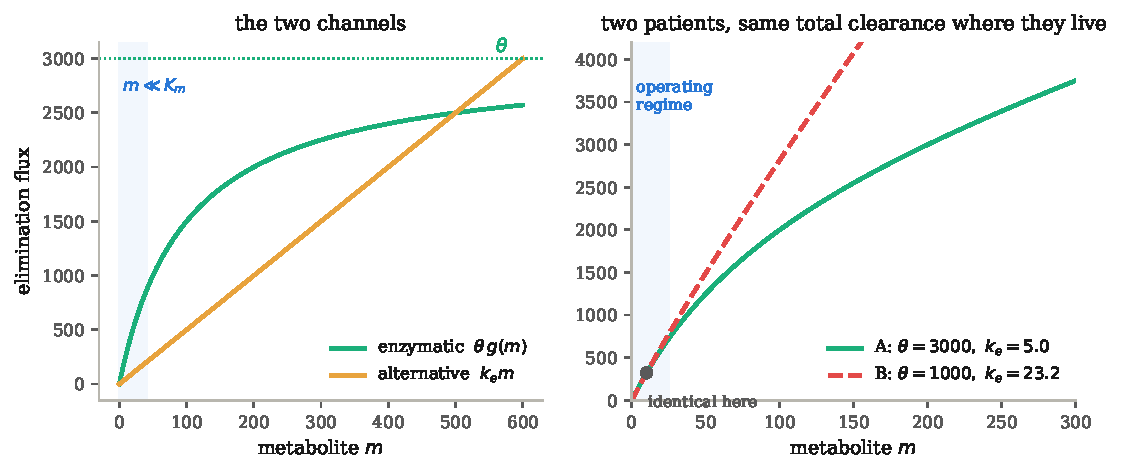
\includegraphics[width=\textwidth]{fig_A1_channels.pdf}
\caption{Left: the two elimination channels. The enzymatic term saturates at $\theta$ while
the alternative term does not, and this difference in functional form is the only thing
distinguishing them in the unforced model. In the shaded band, where clinically stable
patients are maintained, both are approximately linear, which is the difficulty the rest of
this paper is about. Right: two patients agreeing in \emph{both} the value and the slope of
total clearance at the operating point, differing only at second order. They differ
threefold in enzymatic capacity and carry different $K_m$, and no affine fit over a band
around that point tells them apart.}
\label{fig:A1}
\end{figure}


\paragraph{Why the local model is used.} It is not a reduction of the parent. The tangent
to the parent's clearance curve carries an extra term in its intercept, and at the
illustrative constants that term is $374$ against the enzymatic term's $61$, so the
alternative channel owns six-sevenths of an intercept the residual capacity was supposed to
carry. The local model is therefore a different hypothesis about one term, kept because it
is the most favourable case for identification rather than because it approximates
anything, and that is what the conclusion needs: the degeneracy this paper is about appears
in the favourable structure and disappears in the awkward one, so it is not an artefact of a
bad approximation. At matched parameter count the parent carries a degenerate family of the
same dimension, admissible over a sixteen-fold range in $K_m$ and if anything harder to
reject. What closes such a family, in either model, is an independent channel being known,
not curvature in $\alpha$. The reduction hierarchy is verified symbolically and numerically
(supplement, \S S2).

\subsection{Assumptions and their status}
\label{sec:assumed}

\begin{adjustwidth}{-1.0cm}{-1.0cm}
\scriptsize
\def\paramslabel{tab:params}
\def\paramscaption{The constants this paper reasons about, and what each rests on. Three
are from the literature and the rest are chosen for illustration, against what the last
column says. Each row also carries what \emph{kind} of quantity it is, which is a
different question from where it came from, and the species its evidence comes from where
there is one. \textbf{Some conclusions do depend on values in this table}, and the three
that decide a result are priced in the text below. The full registry is \S S2 of the
supplement, which is the authority; this is a selection from it.}
\begin{longtable}{@{}p{0.075\linewidth} p{0.085\linewidth} p{0.22\linewidth} p{0.11\linewidth} p{0.31\linewidth}@{}}
\caption{\paramscaption}\label{\paramslabel}\\
\toprule
\textbf{Symbol} & \textbf{Value} & \textbf{Meaning} & \textbf{Source} & \textbf{What the value rests on} \\
\midrule
\endfirsthead
\multicolumn{5}{@{}l}{\emph{Table \thetable, continued from the previous page}}\\
\toprule
\textbf{Symbol} & \textbf{Value} & \textbf{Meaning} & \textbf{Source} & \textbf{What the value rests on} \\
\midrule
\endhead
\midrule
\multicolumn{5}{r@{}}{\emph{continued on the next page}}\\
\endfoot
\bottomrule
\endlastfoot
\multicolumn{5}{@{}l}{\emph{The local identification model}} \\
\addlinespace[2pt]
$\bar m$ & $10$~$\mu$M & operating point: the level management holds the patient at & \textsc{assumed}\newline \emph{convention}\newline \emph{mouse} & chosen for illustration, and every design quantity is relative to it. The scale is murine~\cite{pkpd_translational}, within $1.6$ of the human newborn cut-off~\cite{dbs_3hp_cutoff} \\
$\theta$ & $3000$~$\mu$M/d & capacity of the enzymatic channel, \textbf{at normal capacity} & \textsc{assumed}\newline \emph{convention} & chosen for illustration as \emph{normal} capacity on the parent model's scale, against residual activity under $5\%$~\cite{pcc_residual_activity} \\
$\theta_{\mathrm{PA}}$ & $\le 150$~$\mu$M/d & capacity in the disease, on the scale of the row above & \textsc{literature}\newline \emph{derived}\newline \emph{human} & residual PCC activity in propionic acidemia is under $5\%$ of control~\cite{pcc_residual_activity}, which on the scale of the row above is $\theta \le 150$ \\
$K_m$ & $100$~$\mu$M & half-saturation of the enzymatic channel, at the plasma level & \textsc{assumed}\newline \emph{effective} & chosen for illustration at $\bar m/K_m = 0.1$, and \emph{not} PCC's in vitro Michaelis constant, $0.29$~mM~\cite{pcc_liver_kinetics}, a different molecule in a different compartment \\
$k_e$ & $5$~d$^{-1}$ & alternative clearance rate constant & \textsc{assumed}\newline \emph{lumped} & \textbf{no independent human measurement}: the translational model has no marker state and no elimination constant~\cite{pkpd_translational}, and the one structure with a first-order marker loss publishes no value~\cite{dose_selection_poster}. Bounded from above by the methylmalonic-acid analogue, $\num{ke_mma}$~d$^{-1}$~\cite{ke_mma_analogue} \\
$\lambda$ & $\ln 2/3.5$~d$^{-1}$ & decay rate of the therapeutic increment & \textsc{literature}\newline \emph{measurable}\newline \emph{mouse, rat, monkey} & the translational model's PK, allometrically scaled from mouse, rat and monkey~\cite{pkpd_translational} \\
$T_{\mathrm{dose}}$ & 14~d & interval between therapeutic doses & \textsc{literature}\newline \emph{measurable}\newline \emph{human} & the biweekly schedule of model-informed dose selection~\cite{dose_selection_poster}; the trial dosed every two or three weeks~\cite{trial_phase12} \\
$D$ & $6000$~$\mu$M/d & size of one therapeutic increment & \textsc{assumed}\newline \emph{calibration}\newline \emph{mouse} & chosen for illustration so the marker falls by about two thirds at peak, against the trial's reported falls~\cite{trial_phase12} \\
$\sigma$ & a family, $\mu$M/d & standard deviation of the ordinate of the fit & \textsc{assumed}\newline \emph{lumped} & deliberately not assigned: nothing here bounds how well the load is recorded, so it is carried as a family indexed by the row below \\
$\mathrm{CV}$ & $5\%$ & analytical variability of the marker assay & \textsc{assumed}\newline \emph{measurable}\newline \emph{human (MMA); mouse} & chosen for illustration. The nearest published repeatability, the breath test's, is between-visit and in methylmalonic acidemia~\cite{breath_test_mma}, so it bounds this from above rather than measuring it \\
$s_{\ln k_e}$ & $0.8$ & sd of the log-normal prior on $k_e$ & \textsc{assumed}\newline \emph{prior width} & chosen for illustration, tighter than the factor of $\num{ke_needed_factor}$ the gate needs, so the gate passes with it in place \\
$\sigma_L/L$ & $5\%$ & relative error in the recorded substrate load & \textsc{assumed}\newline \emph{measurable} & chosen for illustration. Measurable by a weighed intake study; none exists in propionic acidemia, where records are prescriptions rather than intake as eaten \\
\addlinespace
\midrule
\multicolumn{5}{@{}l}{\emph{The parent model and its equilibrium reduction}} \\
\addlinespace[2pt]
$k$ & $1$~d$^{-1}$ & conjugation rate constant, which cancels from the reduced curve & \textsc{assumed}\newline \emph{eliminated}\newline \emph{human} & cancels from the reduced clearance exactly, and nothing fixes it. Chosen for illustration; its cost off equilibrium is bounded in \S S2 \\
\addlinespace
\multicolumn{5}{@{}p{0.92\textwidth}}{\emph{The remaining 11 registered constants are in the supplement, \S S2, with the full provenance of every row in this table.}} \\
\end{longtable}
\end{adjustwidth}


\paragraph{The three rows that decide a result, and what each is worth.} Most of the table
is illustrative in the harmless sense that every conclusion is stated relative to it. Three
rows are not.

\emph{Capacity.} The identifiability results do not turn on $\theta = 3000$, but two
conclusions do. The supplement's local-model section flips a qualitative conclusion across
it, the anchor attenuating at $3000$ and amplifying at the parent model's $300$, and by
Section~\ref{sec:scopeprec} the design's own precision does too.

\emph{Capacity in the disease.} On the monthly record $\operatorname{sd}(\ln\hat\theta)$ is
$0.1699$ at nominal capacity, $1.5830$ at $10\%$ of nominal and $3.0673$ at $5\%$, against
a target of $0.20$. The gate holds only for $\theta$ between $2472$ and $18814$, which is
$82\%$ to $627\%$ of nominal, so the disease sits a factor of $16$ below the band. This is
the row that says who the paper is about, and it is the reason the precision above is an
illustration rather than the result.

\emph{Half-saturation.} This is the tightest cost in the local model after the increment.
Holding the patient managed at $\bar m$ and re-solving the load, the ordinate noise and the
load-bias prior at each $K_m$, $\operatorname{sd}(\ln\hat\theta)$ runs $0.0507$ to $1.3608$
over $K_m$ from $5$ to $1000$~$\mu$M, a factor of $26.8$. It is $0.1699$ at the
illustrative $100$ and crosses the target at $K_m = 124$, so the design has a factor of
$1.24$ of headroom; at the in vitro value the $K_m$ row declines to use, $290$~$\mu$M, it
would be $0.4158$. That headroom is smaller than it reads: across twenty-four intake
records the spread is $0.1684$ to $0.1709$ at $K_m = 100$ and $0.1987$ to $0.2010$ at
$K_m = 124$, so the crossing straddles the target and which side of it a given record falls
on is not settled by the median.

Two consequences of that table are load-bearing and are stated here rather than left to be
inferred.

\begin{remark}[No value of $K_m$ is imported, and none is needed]
\label{rem:no_km}
The in vitro Michaelis constant of PCC is for propionyl-CoA inside the mitochondrion. The
$K_m$ of \eqref{eq:local} is for a plasma marker that is neither that molecule nor in that
compartment, and the two are not interchangeable, so no literature value is used. The
results below do not need one: a prior on $\ln K_m$ twenty times looser than the module's
own changes $\operatorname{sd}(\ln\hat\theta)$ in the fourth decimal, and removing it
entirely changes nothing at all (Section~\ref{sec:designsec}).
\end{remark}

\begin{remark}[The marker, and the observation model both markers need]
\label{sec:marker}
Plasma 3-hydroxypropionate is used. It is the one marker with an endpoint association: a
$50\%$ lower concentration carries a decompensation rate ratio of $0.7$ ($95\%$ CI
$0.6$--$0.9$, $p<0.01$)~\cite{natural_history}, % C49
where 2-methylcitrate has none ($1.0$, $0.7$--$1.3$), and it is not a carnitine conjugate,
so carnitine supplementation does not raise it as it raises C3. But no marker is the PCC
substrate. 3-HP is an overflow metabolite downstream of accumulated propionyl-CoA, and so
is 2-MC. Writing either as the $m$ of \eqref{eq:parent} assumes it tracks the substrate
monotonically: an assumption required identically for either choice, not testable from the
published data, and named first among the limits in Section~\ref{sec:discussion}.
\end{remark}

\subsection{Numerical methods}
\label{sec:numerics}

Every computed trajectory uses an adaptive stiff-capable solver (\texttt{LSODA} or
\texttt{Radau}) at relative tolerance $10^{-8}$ or tighter, and the estimator of
Section~\ref{sec:collapse} does not integrate at all: it uses the closed-form quasi-steady
level of \eqref{eq:alphaqss}. Two tests guard the integration, one halving the step and
asserting the answer moves by less than $10^{-6}$ relative, the other asserting that an
integrated steady state equals the closed-form equilibrium reduction to the same tolerance.
\textbf{Neither measures the validity of the carnitine reduction}, because the first
integrates the local model and the second integrates the \emph{reduced} system and compares
it against the algebraic root of the same reduced clearance, so the two-state system appears
in neither. What licenses the reduction is the identity of \S\ref{sec:reduction}, and what
bounds its cost off equilibrium is the $k$ row of the supplement's registry, \S S2.

Every stochastic result uses \texttt{numpy.random.default\_rng} with an explicit seed named
at the call site, and each quoted precision is a median over $24$ intake records with its
range beside it unless stated otherwise. Fitted ensembles are cached on
$(\text{design}, \sigma, \mathrm{CV}, \text{reps}, \text{seed})$, so the same design is
fitted once and reused across a sweep.

\clearpage
\section{The excitation condition: what a trajectory has to do}
\label{sec:excitation}
%==========================================================================

\emph{Everything so far says what a record confined to a band cannot deliver. This
section says what a record would have to do instead, and it is the link between the
obstruction and the data specification.}

\subsection{The parametrisation, pinned}
\label{sec:pinned}

Nothing below can be proved until one choice is made explicit, because the two natural
parametrisations give different statements. The enzymatic flux is written
\begin{equation}
\theta\, g(m), \qquad g(m) = \frac{m}{K_m+m},
\label{eq:pin}
\end{equation}
with $\theta$ \emph{absorbing} the maximal velocity: $\theta$ \emph{is} the patient's
residual $V_{\max}$, not a fraction of a population $V_{\max}$. Carrying the two
separately, as $V_{\max}\theta\, g(m)$ with $\theta \in [0,1]$, adds a parameter that no
excursion separates, since only the product multiplies $g$. Splitting them requires an
anchor outside the marker, and the $1$-$^{13}$C-propionate breath test is what such an
anchor looks like~\cite{breath_test_mma}. % C48
The dynamic model is then
\begin{equation}
\dot m \;=\; L(t) + L_0 \;-\; \bigl(\theta + \Delta(t)\bigr) g(m) \;-\; k_e\, m ,
\label{eq:dyn}
\end{equation}
with $L$ the recorded component of the propiogenic load, $L_0$ its unrecorded component
carried as an unknown constant, and $\Delta$ the therapeutic increment, known from the
dosing schedule.

\subsection{Both ends are degenerate, and they fail differently}

\begin{proposition}[Two degeneracies]
\label{prop:excitation}
In \eqref{eq:dyn} with $(\theta, K_m, k_e, L_0)$ unknown:
\begin{enumerate}[leftmargin=*, itemsep=2pt]
\item \textbf{Below the half-saturation level.} As $m/K_m \to 0$, $g(m) \to m/K_m$ and
total clearance collapses to $\left(\theta/K_m + k_e\right) m$. Three of the four
sensitivity directions become proportional to $m$, so only the lumped ratio
$\theta/K_m + k_e$ is identifiable and $\theta$, $K_m$ and $k_e$ are not separable.
\item \textbf{Above it.} As $m/K_m \to \infty$, $g(m) \to 1$ and \eqref{eq:dyn} becomes
$\dot m = L(t) + L_0 - \theta - k_e m$. \textbf{$\theta$ enters only through
$L_0 - \theta$}, so with $L_0$ unknown the residual capacity and the unrecorded load are
confounded and cannot be separated from the marker trajectory at all.
\end{enumerate}
\end{proposition}

\begin{proof}[Argument]
Both are limits of the sensitivity matrix. Writing the four columns as derivatives of the
ordinate with respect to $(\ln\theta, \ln K_m, \ln k_e, L_0)$,
\[
\Bigl(\theta g(m),\;\; -\theta K_m \tfrac{m}{(K_m+m)^2},\;\; k_e m, \;\; 1 \Bigr),
\]
the first three tend to $\bigl(\theta m/K_m,\, -\theta m/K_m,\, k_e m\bigr)$ as
$m/K_m \to 0$, all proportional to $m$ and hence of rank one together with the constant
fourth; and to $(\theta,\, 0,\, k_e m)$ as $m/K_m \to \infty$, where the first coincides
with the fourth. Rank two at both ends.
\end{proof}

\textbf{The two failures are not equally survivable.} At the low end a decomposition is
lost while the clearance itself stays constrained: the data still say what the patient
eliminates, they do not say through which channel. At the high end the target parameter is
lost against a quantity nobody records. The earlier phrasing of this note --- ``below $K_m$
only the lumped ratio, above $K_m$ only the product'' --- was wrong in the second clause,
and wrong in the direction that matters.

\begin{remark}[Which makes the load record load-bearing]
\label{rem:load_bearing}
Proposition~\ref{prop:excitation}(2) is conditional on $L_0$ being unknown. If the load
were recorded exactly, saturation would be the \emph{best} place to measure, not the worst:
$C(m) \to \theta + k_e m$ and the intercept of that line is $\theta$ outright, with no
extrapolation and no $K_m$. Figure~\ref{fig:D1}~(right) draws both cases, and they differ
qualitatively: with the load known, $\operatorname{sd}(\ln\hat\theta)$ falls monotonically
as the patient is carried up the curve; with it partly unrecorded, the optimum is
\emph{interior}.

So load-recording precision is not a mechanical detail to be tidied up at the end. It is
what creates the upper obstruction, and it is therefore the first thing on the data
specification of Section~\ref{sec:spec}.
\end{remark}

\subsection{Identifiability comes from curvature, and there is a closed form}

Since both ends are flat, what separates the parameters is the \emph{change} in the
saturation across the visited range. The ratio of the $K_m$ sensitivity to the $\theta$
sensitivity is
\begin{equation}
\frac{\partial C/\partial \ln K_m}{\partial C/\partial \ln \theta}
\;=\; -\bigl(1 - g(m)\bigr) \;=\; -\varphi(m),
\qquad \varphi(m) = \frac{K_m}{K_m + m},
\label{eq:phi}
\end{equation}
and the ratio of the $k_e$ sensitivity to it is $(k_e/\theta)(K_m + m)$, which is affine in
$m$ and which any excursion excites. It is $\varphi$ that is flat at both ends, so the
quantity a design has to buy is the drop in $\varphi$ across the band:
\begin{equation}
E \;=\; \varphi(m_{\min}) - \varphi(m_{\max})
\;=\; \frac{K_m\,(m_{\max} - m_{\min})}{(K_m + m_{\min})(K_m + m_{\max})} .
\label{eq:E}
\end{equation}

\begin{proposition}[The excitation is maximised straddling $K_m$]
\label{prop:straddle}
Fix the fold range $r = m_{\max}/m_{\min} > 1$. Then $E$ is maximised at
\begin{equation}
m_{\min} = \frac{K_m}{\sqrt r}, \qquad m_{\max} = K_m \sqrt r,
\qquad\text{that is}\qquad \sqrt{m_{\min} m_{\max}} = K_m ,
\label{eq:straddle}
\end{equation}
and there
\begin{equation}
E_{\max}(r) \;=\; \frac{\sqrt r - 1}{\sqrt r + 1},
\qquad\text{so a required $E$ needs}\qquad
r \;\ge\; \left(\frac{1+E}{1-E}\right)^{\!2} .
\label{eq:Emax}
\end{equation}
\end{proposition}

\begin{proof}
Put $x = m_{\min}/K_m$, so $E = (1+x)^{-1} - (1+rx)^{-1}$. Then
$\partial E/\partial x = -(1+x)^{-2} + r(1+rx)^{-2}$, which vanishes when
$\sqrt r\,(1+x) = 1 + rx$, that is at $x = 1/\sqrt r$. Substituting gives
$E_{\max} = \sqrt r/(\sqrt r + 1) - 1/(1 + \sqrt r)$, which is \eqref{eq:Emax}, and
inverting it gives the requirement on $r$.
\end{proof}

\textbf{The requirement is a band around $K_m$, not a threshold above it.} That is the
correction this section exists to make, and it changes what a protocol should ask for. A
band of a given fold range placed a decade below $K_m$ delivers a fraction of what the same
fold range delivers straddling it: at $r = 2$, the band the illustrative patient is held in
gives $E = 0.058$ against a possible $0.172$, a factor of three thrown away by placement
alone. Across four decades of operating point the penalty is far larger than that, because
$\operatorname{sd}(\ln\hat\theta)$ depends on placement more steeply than $E$ does:
\textbf{at the operating point this note's patient is managed to, it is about $2\,100$ times
its best} (Figure~\ref{fig:D1}).

\begin{figure}[htbp]
\centering
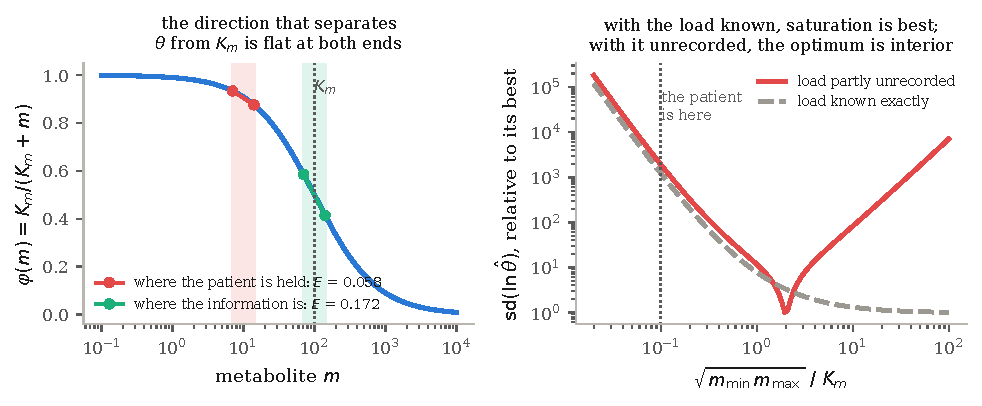
\includegraphics[width=\textwidth]{fig_D1_excitation.pdf}
\caption{The excitation condition. \textbf{Left:} $\varphi(m) = K_m/(K_m+m)$, the direction
that separates $\theta$ from $K_m$. It is flat at both ends of the saturation curve, so the
information a band carries is the \emph{drop} in $\varphi$ across it,
\eqref{eq:E}. The two shaded bands have the same fold range and differ only in where they
sit. \textbf{Right:} the price of sitting in the wrong place, as
$\operatorname{sd}(\ln\hat\theta)$ against the geometric centre of the band. With the load
known exactly the curve is monotone and saturation is the best place to measure; with the
load partly unrecorded the optimum is interior, because
Proposition~\ref{prop:excitation}(2) then bites. The dotted line is where clinical
management holds the patient.}
\label{fig:D1}
\end{figure}

\begin{remark}[Two ways to buy the same information, and only one of them is available]
\label{rem:two_buys}
Equation \eqref{eq:Emax} says a required excitation can be met either by a wide band
wherever the patient is, or by a narrow band placed correctly. The two are not
interchangeable clinically. Reaching the neighbourhood of $K_m$ means carrying the marker
to roughly twenty times its managed level, which is a decompensation; buying the same
information from the operating point instead needs a fold range of order ten, which is also
a decompensation, reached from below. \textbf{The safety constraint is on the level, and both
routes violate it.} What separates them is that the first is cheap in width and the second
is cheap in level, so a protocol that has any room at all should spend it on placement
rather than on duration.
\end{remark}

\vspace{0.5em}
\hrule
\vspace{1em}

%==========================================================================

\section{The design: where the excitation can be bought, and what it decides}
\label{sec:designsec}
%==========================================================================

\emph{Section~\ref{sec:excitation} says what a trajectory has to do. This section asks
what the accessible trajectories actually do, and what decision the answer supports.}

\subsection{What does not collapse, stays --- and what does, and why}
\label{sec:collapse}

The estimator here is the exact information filter for constant parameters,
\begin{equation}
P_k^{-1} \;=\; P_0^{-1} \;+\; \sum_{i \le k} \frac{q(m_i, \Delta_i)\,q(m_i, \Delta_i)^{\!\top}}{\sigma^2},
\label{eq:infofilter}
\end{equation}
on the augmented coordinates $(\ln\theta, \ln K_m, L_0, \ln k_e)$, none of which carries
dynamics. \textbf{There is no process noise on $\theta$, and that is a construction rather
than a setting.} A random walk on $\theta$ manufactures a finite stationary covariance in a
direction the data may never see, which is precisely the error this note exists to warn
about; with \eqref{eq:infofilter}, what does not collapse stays visibly uncollapsed.

\paragraph{The footing, stated once and used everywhere.} Four choices decide every number
in this section, and earlier drafts of this note did not hold them fixed.
\begin{enumerate}[leftmargin=*, itemsep=2pt]
\item \textbf{$q$ carries the increment}, as \eqref{eq:columns} requires. A design is
\emph{not} fully described by the levels it visits: two samples at the same level under
different $\Delta$ carry different information, and that is the whole of
Section~\ref{sec:therapychannel}.
\item \textbf{$\theta$ and $K_m$ are free.} No prior is placed on either. Stripping the
priors one at a time shows that the $K_m$ prior does no work at all --- the accessible
design gives $0.1474$ with it and $0.1474$ without it, and still $0.1474$ at a prior
twenty times looser --- so nothing here depends on knowing $K_m$, which
Remark~\ref{rem:no_km} forbids.
\item \textbf{$k_e$ carries a log-prior of $0.8$}, a factor of $2.2$, and it is the only
prior that does any work: removing it takes the same design from $0.1474$ to $0.6451$. The
gate needs $k_e$ within a factor of $2.95$, which is the one thing this note asks the
literature for.
\item \textbf{Intake varies day to day at a $10\%$ coefficient of variation, and is
recorded to $5\%$.} By Proposition~\ref{prop:rank} a perfectly steady load is the exactly
singular case, so the variability is not noise to be averaged away.
\end{enumerate}

An extended Kalman filter on the joint state was written first and is not used, for a
reason worth recording. The marker's time constant is
$\bigl((\theta+\Delta) g'(\bar m) + k_e\bigr)^{-1}$, which is $0.81$ hours at the
illustrative values, against a therapeutic increment decaying with a half-life of $3.5$
days: a separation of $104$. The marker is therefore in quasi-steady state at every
sampling instant a clinic could use and \eqref{eq:infofilter} is exact rather than
approximate. The code measures the separation rather than asserting it, and returns one
number a protocol needs: after a dose the marker is within $5\%$ of quasi-steady in $0.91$
hours and tracks to within $5\%$ thereafter, so a sample drawn inside that first hour is
not a steady state and does not belong in a steady-state fit.

\begin{figure}[htbp]
\centering
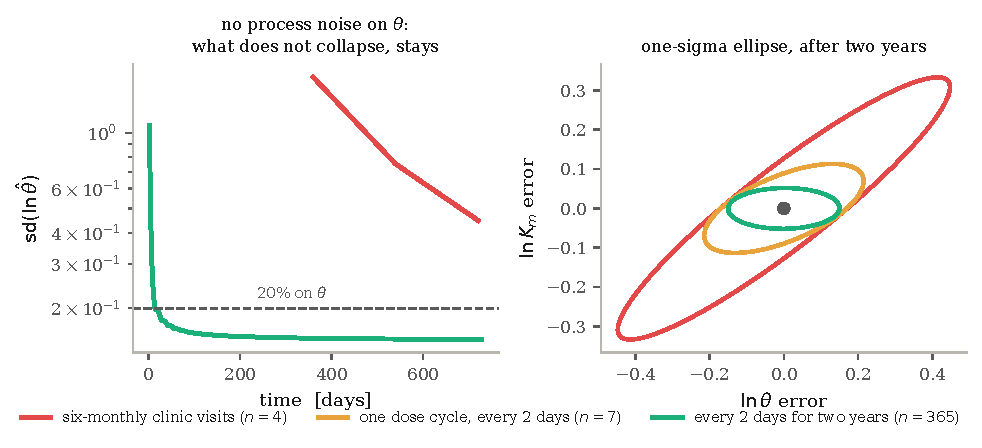
\includegraphics[width=\textwidth]{fig_D2_collapse.pdf}
\caption{Three sampling designs under the biweekly dosing schedule, over two years.
\textbf{Left:} $\operatorname{sd}(\ln\hat\theta)$ as samples arrive. \textbf{Right:} the
one-sigma ellipse in $(\ln\theta, \ln K_m)$ at the end. What separates the designs is how
much of the dose cycle they see, not how many samples they take.}
\label{fig:D2}
\end{figure}

\begin{adjustwidth}{-1.4cm}{-1.4cm}
\begin{table}[htbp]
\centering
\footnotesize
\caption{\label{tab:designs}What each design delivers. Bold is inside the $20\%$ target.
The fourth column is the range of the therapeutic increment the design actually sees, and
it, rather than $n$, is what orders the table. The last column is the same design evaluated
with the increment dropped from the sensitivity while still being used to generate the
levels, which is what earlier drafts of this note reported.}
\begin{tabular}{@{}llllll@{}}
\toprule
\textbf{design} & \textbf{$n$} & \textbf{levels visited} & \textbf{range of $\Delta/\theta$} & \textbf{$\operatorname{sd}(\ln\hat\theta)$} & \textbf{$\operatorname{corr}(\ln\hat\theta, \ln \hat K_m)$} \\
\midrule
six-monthly clinic visits & 4 & $5.76$--$10.34$ & $0.45$ & 0.4570\,\scriptsize$[0.4121, 0.5097]$ & $+0.9278$ \\
one dose cycle, every two days & 7 & $3.28$--$7.79$ & $1.81$ & 0.2162\,\scriptsize$[0.2053, 0.2300]$ & $+0.6137$ \\
\textbf{monthly, across dose cycles} & 25 & $2.81$--$9.47$ & $1.84$ & \textbf{0.1699}\,\scriptsize$[0.1684, 0.1709]$ & $+0.3356$ \\
two-monthly, across dose cycles & 13 & $3.28$--$9.70$ & $1.94$ & \textbf{0.1876}\,\scriptsize$[0.1839, 0.1939]$ & $+0.4711$ \\
every two days for two years & 365 & $2.49$--$10.47$ & $1.95$ & \textbf{0.1500}\,\scriptsize$[0.1498, 0.1501]$ & $+0.0327$ \\
\emph{fortnightly: the dose interval itself} & 53 & $2.39$--$4.53$ & $0.13$ & 4.5845\,\scriptsize$[3.5050, 5.6362]$ & $+0.9990$ \\
\emph{the same $365$ straddling $K_m$} & 365 & $50.00$--$200.00$ & $1.95$ & \textbf{0.0157}\,\scriptsize$[0.0157, 0.0157]$ & $+0.2055$ \\
\bottomrule
\end{tabular}
% theta and K_m free; priors only on ln k_e and the load record. Medians over 24 intake records, range in brackets.
\end{table}
\end{adjustwidth}

\textbf{The gate passes, and it passes on ordinary outpatient care.} Sampling monthly
across dose cycles for two years --- twenty-five draws, no excursion, no admission ---
reaches $\operatorname{sd}(\ln\hat\theta) = 0.170$, inside the $20\%$ target. Two-monthly
sampling, thirteen draws, reaches $0.187$ and also passes. Six-monthly visits reach
$0.418$ and do not.

\textbf{What separates them is not $n$.} Two-monthly sampling passes with thirteen samples
while fortnightly sampling fails with fifty-three. Read the fourth column instead: the
designs that pass are the ones that see the increment vary, and the ones that fail are the
ones that do not. Six-monthly visits catch a range of $\Delta/\theta$ of $0.45$;
two-monthly visits catch $1.94$.

\begin{remark}[Do not sample at the dose interval. This is the sharpest rule in the note.]
\label{rem:aliasing}
The fortnightly row of Table~\ref{tab:designs} is a catastrophe, and it is a
\emph{designed} catastrophe rather than bad luck. The dose interval is fourteen days, so
sampling every fourteen days lands every draw at the same phase of every cycle. The range
of $\Delta/\theta$ collapses from $1.95$ to $0.13$, the correlation between $\ln\theta$ and
$\ln K_m$ returns to $+0.998$, and $\operatorname{sd}(\ln\hat\theta)$ goes to $3.51$. The
same happens at twenty-eight days, and at any multiple.

\textbf{Moving the schedule by half a day fixes it}: sampling every $14.5$ days gives
$0.161$. A factor of twenty-two in the precision of the answer turns on a choice a protocol
writer would make for administrative convenience, and would currently make the wrong way,
because ``sample on dosing days'' is the obvious thing to write.
\end{remark}

\textbf{Three more things in that table are worth reading against what this note used to
say.}

\begin{enumerate}[leftmargin=*, itemsep=3pt]
\item \textbf{The last column is the error.} With the increment dropped from the
sensitivity, every accessible design sits between $1.0$ and $9.4$ and none of them
collapses, which is what earlier drafts reported as the result. The correction is checked
against a finite difference of the integrated dynamics in two independent ways, on two
integrators over two spans (Appendix~\ref{sec:repro}); the uncorrected column is wrong by
up to $64\%$ of itself at the top of a dose cycle.
\item \textbf{Placement still helps, and by a factor of nine rather than a hundred.} The
same $365$ samples placed to straddle $K_m$ reach $0.0157$ against $0.1499$. The straddling
design remains unavailable for the reasons of Section~\ref{sec:excursion_table}, so this is
a statement about what is being given up, not a recommendation.
\item \textbf{One dose cycle of seven samples does not do it.} It reaches $0.219$ and has a
floor there: no improvement in how well the increment is known brings it inside the target,
because what limits it is the design and not the product. An earlier report of this work
claimed that single cycle passed; it did so only with $k_e$ held known, and the claim is
withdrawn in \texttt{REVIEW\_LOG.md} rather than deleted.
\end{enumerate}

\textbf{And the load record behaves in the way Proposition~\ref{prop:rank} says, not the
way this note used to assume.} Recording the load ten times better --- to $0.5\%$, which
nobody can do --- moves the dense design by about one per cent. That retires the claim that
load-record \emph{precision} is the binding design variable. What the record has to contain
instead is \emph{variation}: by Proposition~\ref{prop:rank} a perfectly steady intake is the
exactly singular case, and half a per cent of day-to-day variability restores full rank.

\begin{remark}[What the filter claims, and what a prior-free fit says instead]
\label{rem:priorfree}
Table~\ref{tab:designs} reports posterior standard deviations under one prior, and that
prior is load-bearing. With \emph{no} prior at all --- $k_e$ free as well --- the same
two-daily design gives $\operatorname{sd}(\ln\hat\theta) = 1.03$, and a prior-free
nonlinear least squares started half a decade from the truth does worse still, because
along the near-null direction of Proposition~\ref{prop:rank} the gradient is third order
and a started-away optimiser does not climb back. \textbf{So the honest claim is
conditional and is stated as such: this design identifies $\theta$ to better than $20\%$
\emph{given} $k_e$ within a factor of about three, and does not identify it at all
without.} What survives unconditionally is the comparison --- carrying the increment is
worth between one and two orders of magnitude on every design in the table, prior-free ---
and it is the comparison, not the absolute number, that the data specification rests on.
\end{remark}

\subsection{Where the excitation could come from}
\label{sec:excursion_table}

Each accessible source of variation moves the marker by a known amount, in a known
direction, from a known place. Table~\ref{tab:excursion} evaluates \eqref{eq:E} on each.

\begin{adjustwidth}{-1.0cm}{-1.0cm}
\begin{table}[htbp]
\centering
\footnotesize
\caption{\label{tab:excursion}Excitation available from each source, against the
$E \approx 0.50$ the decision requires. Direction matters: the curvature is at high $m$, and
most of what a chart contains moves the patient the other way. The last column is how much
of the excitation a band of that fold range \emph{could} have delivered if it had straddled
$K_m$, so it separates being too narrow from being in the wrong place.}
\begin{tabular}{@{}p{0.29\textwidth}lllllll@{}}
\toprule
\textbf{source} & \textbf{$m$ range} & \textbf{fold} & \textbf{direction} & \textbf{$\sqrt{m_{\min}m_{\max}}/K_m$} & \textbf{$E$} & \textbf{$E_{\max}(r)$} & \textbf{frac.\ of $E_{\max}$} \\
\midrule
inter-dose recovery, biweekly schedule & 3.40--8.9 & 2.6$\times$ & down & 0.055 & 0.0489 & 0.2363 & 0.21 \\
carnitine dose step (quasi-exogenous) & 3.00--10.0 & 3.3$\times$ & down & 0.055 & 0.0618 & 0.2922 & 0.21 \\
cyclical intestinal antibiotics & 6.00--10.0 & 1.7$\times$ & down & 0.077 & 0.0343 & 0.1270 & 0.27 \\
carnitine supply interruption & 10.00--16.0 & 1.6$\times$ & up & 0.126 & 0.0470 & 0.1170 & 0.40 \\
decompensation and recovery & 10.00--80.0 & 8.0$\times$ & up & 0.283 & 0.3535 & 0.4776 & 0.74 \\
labelled-propionate bolus (not administered) & 10.00--20.0 & 2.0$\times$ & up & 0.141 & 0.0758 & 0.1716 & 0.44 \\
\bottomrule
\end{tabular}
% E is the excitation the band delivers; E_max(r) is the most a band of that fold range could deliver if it straddled K_m
\end{table}
\end{adjustwidth}

Three readings.

\begin{enumerate}[leftmargin=*, itemsep=3pt]
\item \textbf{Everything routine is in the wrong place, not merely too narrow.} The
inter-dose recovery, the carnitine dose steps and the cyclical antibiotics all deliver
between a fifth and a quarter of what their own fold range could deliver, because they
happen an order of magnitude below $K_m$. Widening them does not fix that.
\item \textbf{Only a decompensation gets close, and it is still short.} An excursion from
the operating point to eight times it reaches $E = 0.35$ against the $0.50$ required, and it
does so at $74\%$ of what that fold range could deliver, because it at least moves towards
$K_m$. \textbf{The excitation the decision needs is available only from the event the
treatment exists to prevent}, and even then not in full.
\item \textbf{A labelled-propionate bolus is the one designed source, and it is small.}
Doubling the marker from the operating point reaches $E = 0.076$. Its value is not the
excitation it supplies but that it measures capacity on a different axis entirely, which is
the subject of Section~\ref{sec:validation}.
\end{enumerate}

\subsection{The estimand is a decision, and the decision survives what the parameter does not}
\label{sec:decision}

Confidence intervals on $\theta$ are the wrong output. The clinical question is the
\emph{sign} of $\mu = \theta - \thc$, and its two errors are not interchangeable: treating a
patient who does not need it costs an infusion and a venous line, and failing to treat one
who does costs a decompensation. Figure~\ref{fig:D3} is the operating characteristic of that
decision.

\begin{figure}[htbp]
\centering
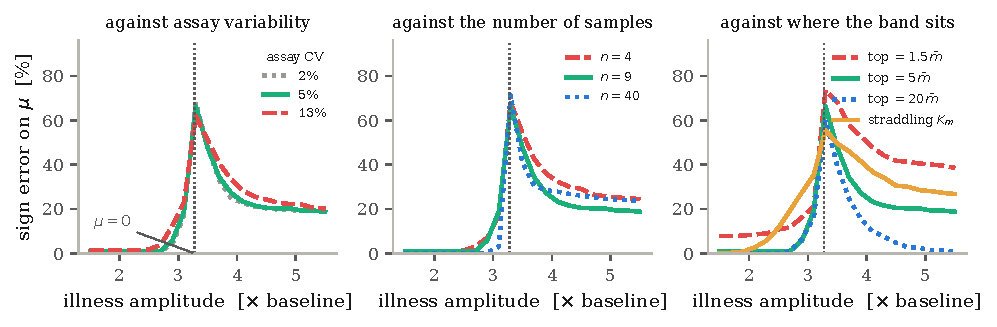
\includegraphics[width=\textwidth]{fig_D3_decision.pdf}
\caption{The probability of getting the sign of $\mu$ wrong, by simulation, as a patient of
fixed biology is swept across the decision boundary by the illness amplitude. Left of the
dotted line the error is a patient treated who did not need it; right of it, a patient left
untreated who did. Each panel varies one thing a protocol controls.}
\label{fig:D3}
\end{figure}

\begin{center}
\footnotesize
\begin{tabular}{@{}rrlrr@{}}
\toprule
\textbf{illness} & $\mu$ & \textbf{which error} & \textbf{simulated} &
\textbf{a delta method would say} \\
\midrule
$1.50\times$ & $+2006$ & treat unneeded & $0.2\%$  & $39.5\%$ \\
$2.50\times$ & $+876$  & treat unneeded & $0.2\%$  & $38.8\%$ \\
$2.98\times$ & $+339$  & treat unneeded & $6.0\%$  & $36.1\%$ \\
\addlinespace
$3.58\times$ & $-339$  & fail to treat  & $\mathbf{52.5\%}$ & $42.3\%$ \\
$4.00\times$ & $-818$  & fail to treat  & $31.8\%$ & $41.1\%$ \\
$5.50\times$ & $-2513$ & fail to treat  & $26.0\%$ & $40.4\%$ \\
\bottomrule
\end{tabular}
\end{center}

\textbf{The two errors are not the same size, and the larger one is the one that costs a
patient a decompensation.} At equal distance from the boundary --- $|\mu| = 339$ on either
side --- the simulated error is $6\%$ for treating a patient who did not need it and $53\%$
for failing to treat one who did. The asymmetry does not close with distance: at
$|\mu| = 2513$ on the unsafe side the error is still $26\%$, where at $|\mu| = 2006$ on the
safe side it is $0.2\%$. \textbf{The estimator fails towards declaring patients safe.} The
mechanism is already in this note: by Remark~\ref{rem:eiv} the abscissa noise inflates
$\hat a$ and hence $\hat\theta$, and $\hat\mu = \hat\theta - \thc$ inherits that bias
whole.

The simulated error exceeds $10\%$ for every illness amplitude from $3.10\times$ baseline
upward, which is the whole region at and beyond the decision boundary at $3.28\times$. A
protocol reporting this design's answer would be reporting a test that is nearly reliable
where it does not matter and close to a coin toss where it does.

\textbf{What excursion would fix it, and whether one exists.} Asking the same question of a
patient $30\%$ below the threshold, the simulated sign error falls from $36\%$ at a
two-fold excursion to $10\%$ at twenty-fold and then \emph{plateaus near $6\%$}: past about
forty-fold, more excursion buys nothing. The plateau is the load-bias degeneracy of
Proposition~\ref{prop:excitation}(2), which excursion does not touch. So there is no
excursion, survivable or otherwise, that delivers a $5\%$ sign error at this load record ---
and the requirement that does bite, a twenty-fold excursion for a one-in-ten error, is a
severe decompensation. Table~\ref{tab:spec} carries the whole curve.

\begin{remark}[Why this is simulated and not propagated]
\label{rem:no_delta}
A delta-method calculation, propagating the estimator's covariance to $\mu$ and reporting
$\Phi(-|\mu|/\operatorname{sd}(\hat\mu))$, is available and is wrong here, in a way that
matters. At the accessible design $\operatorname{sd}(\hat\mu)/|\mu| = 3.7$, so a Gaussian
of that width crosses zero about $39\%$ of the time. Simulating the same model instead,
$\hat\theta$ ranges over three orders of magnitude across replicates --- the design really
is that bad --- and $\hat\mu$ never changes sign.

The two disagree because $\hat\mu$ is not symmetric about $\mu$. The design's near-null
direction is very nearly the direction along which $\mu$ is monotone and of one sign, so the
sampling distribution of $\hat\mu$ is heavily skewed and does not cross zero anything like
as often as its standard deviation suggests. \textbf{That is the margin theorem of
\eqref{eq:mufibre} showing up in the estimator}, and taking the Gaussian tail at face value
would throw away the one favourable result this note has. Both numbers are reported by the
code so that the gap stays visible.
\end{remark}

\vspace{0.5em}
\hrule
\vspace{1em}

%==========================================================================

\clearpage
\section{The data specification}
\label{sec:spec}
%==========================================================================

\emph{Every row is generated from the model code and is a consequence of something proved
above. It has two tiers, and the order is not cosmetic: Tier~1 is a single measurement
nobody has published, and until it reports there is no defensible answer to the question
Tier~2 asks.}

\begin{adjustwidth}{-1.4cm}{-1.4cm}
\begin{table}[htbp]
\centering
\footnotesize
\caption{\label{tab:spec}What a record would have to contain for $\theta$ to be
identifiable. Quantities are in observable units, not multiples of $K_m$, because $K_m$ is
not known --- and by the last row does not need to be.}
\begin{tabular}{@{}lll@{}}
\toprule
\textbf{quantity} & \textbf{requirement} & \textbf{why} \\
\midrule
marker & plasma 3-hydroxypropionate & endpoint association (RR 0.7, 95\% CI 0.6--0.9) and immunity to the carnitine sign reversal that disqualifies C3 \\
second channel & $n$-propionylglycine, optional & a glycine conjugate, so carnitine does not raise it. Worth adding only after the load record is good enough for the assay term to bind \\
sampling interval & $\le$ 4 days through any excursion; 14-day cycles otherwise & the inter-dose recovery is the only excursion a fixed schedule supplies, and six-monthly visits do not resolve it \\
excursion, required & $m$ to reach 14.6$\,\bar m$ from the operating point, or a band of fold range 9.1 straddling $K_m$ & the excitation condition. Below it the band is degenerate in the lumped ratio; above $K_m$ it is degenerate in $\theta$ against the load \\
excursion, available & inter-dose recovery reaches a fold of about 2.6, downward & so the required excursion is not available from the schedule alone \\
load record & protein intake to $\le 5\%$, dated, with enteral and parenteral sources separated & the load's unrecorded component is what makes saturation degenerate, and it is the noise term a marker panel cannot average away \\
labelled-propionate test & once per patient at entry, repeated at any dose change & the only measurement that anchors capacity independently of level. Reference precision 12.8\% in patients \\
assay precision & coefficient of variation $\le$ 5\%, reported on the log scale & a constant CV is a constant variance on the log scale, which is the only scale on which $\sigma$ has unambiguous units \\
instrument events & $n \ge 77$ per patient for $20\%$ on $\theta$ & the floor is set by $\sigma$ alone and no excursion beats it \\
cohort & $N \ge 3,121$ to place the fraction with $\mu<0$ within $\pm 10$ points, at the accessible design's sign error of 41\% near the boundary & sized on the sign error of $\mu$, not on a confidence interval for $\theta$. Per-patient misclassification attenuates the fraction towards one half and inflates the corrected variance by $(1-2p)^{-2}$, which diverges as $p \to 1/2$ \\
the asymmetry & the two errors are not equal and the costly one is larger & at equal $|\mu|$ either side of the boundary the simulated error is $6\%$ for treating a patient who did not need it and $53\%$ for failing to treat one who did. The design fails towards declaring patients safe \\
\bottomrule
\end{tabular}
% the terminal specification; every row is generated
\end{table}
\end{adjustwidth}

\subsection{Tier 1: the measurement the method's feasibility turns on}
\label{sec:tier1}

\textbf{What to run.} One cohort, two $1$-$^{13}$C-propionate breath tests bracketing a
single dose, on one day. The quantity measured is the repeatability of the assay
\emph{within a day and within a state}, which is what a pre/post pair around a dose depends
on.

\textbf{Why it is first.} By Section~\ref{sec:excitation} the therapy channel is what makes
$\theta$ identifiable, and \eqref{eq:dosereq} is stated in units of $\theta$: the ratio
$\Delta/\theta$ is only as well known as $\Delta$ is. Section~\ref{sec:designsec} turns
that into one number --- the delivered increment must be characterised to about $12\%$ for
monthly sampling to reach the $20\%$ target on $\theta$. \textbf{Everything the therapy
channel buys is conditional on that, and it has never been measured.}

\textbf{What is published is an upper bound, and it is not the quantity needed.} The only
repeatability data for this assay~\cite{breath_test_mma} % C48
are between-visit: controls repeated at one- to three-week intervals, and fifteen
\emph{mut} patients at separate visits \emph{two months to four years apart}, with the
authors naming changing renal status and varying $V\mathrm{CO}_2$ as causes. The Results
give $14.02 \pm 12.86\%$ with a range of $0.39$ to $50.84\%$; the abstract's widely quoted
$12.8\%$ is the standard deviation of the per-subject coefficients, not their mean. And the
cohort is methylmalonic acidemia, not propionic acidemia, where the block sits at PCC
itself.

Between-visit variation is an \emph{upper bound} on same-day error, because it contains
drift a same-day pair removes, and the bound sits close to the requirement. \textbf{But a
bound that happens to sit near a threshold is not a measurement of it}, and a per-subject
range reaching $50.8\%$ cannot be applied to an individual. Tier~1 replaces an inference
with a number.

\subsection{Tier 2: conditional on Tier 1, and then it is a small study}

\paragraph{Cover the dose cycle; do not chase the marker.} Monthly draws across dose cycles
for two years reach the target, and two-monthly draws --- thirteen over two years --- also
reach it. This is ordinary outpatient blood work. What buys the information is the
\emph{phase}, not the rate: a schedule that sees the increment vary identifies $\theta$ and
one that does not, does not, whatever its density.

\paragraph{And one hard exclusion a protocol would currently get wrong.}
\textbf{Do not sample on dosing days, or at any multiple of the dose interval}
(Remark~\ref{rem:aliasing}). ``Draw bloods when the patient attends for dosing'' is the
natural thing to write and it is the one schedule that destroys the result: every draw
lands at the same phase, the range of $\Delta/\theta$ collapses from $1.95$ to $0.13$, and
$\operatorname{sd}(\ln\hat\theta)$ goes from $0.17$ to $3.51$. Moving the schedule half a
day recovers it.

\paragraph{The load record: ordinary precision, and keep the variation.} Recording intake
twenty times more precisely buys about six per cent, so precision is not the binding
variable. The variability is subtler and enters twice. By Proposition~\ref{prop:rank} a
perfectly steady load makes the design exactly rank deficient, and that null direction must
be filled by something; as the specification stands it is filled by the $5\%$ prior on the
load bias, and only real day-to-day variation lets the \emph{data} fill it instead. So
``record intake as eaten, do not smooth it'' is the difference between a result the data
support and one a prior supports. It costs nothing: it is an instruction to omit a
data-cleaning step, not to add a measurement.

\paragraph{$k_e$, and nothing else, is assumed.} The result needs the non-enzymatic
clearance within a factor of about three, which the literature supplies; no measurement
programme is proposed for it. $K_m$ is assumed at nothing: a prior twenty times looser
leaves every number unchanged, which is what Remark~\ref{rem:no_km} demanded.

\subsection{What is excluded, and what is not promised}

Two acquisitions an earlier draft asked for are struck out. \textbf{High-frequency sampling
at a fixed operating point} buys nothing: two-monthly sampling with thirteen draws beats
fortnightly sampling with fifty-three, because the first sees the dose cycle and the second
is aliased against it. \textbf{Decompensation records} are excluded twice over --- the
excursion is not observed at the magnitude required, and by Section~\ref{sec:discussion}
the model does not hold in that regime.

\textbf{And the specification does not promise a decision.} It buys an identified $\theta$.
Section~\ref{sec:decision} shows that the sign of the margin does not follow from it, for
reasons that are not about the data, and Section~\ref{sec:scope} shows that $\theta$ itself
stops being recoverable in the patients the question matters most for. A protocol written
from this page should report $\hat\theta$ with its interval and should not be read as a
rule for escalating an individual patient.

\vspace{0.5em}
\hrule
\vspace{1em}

%==========================================================================

\section{Limits of recoverability}
\label{sec:scope}
%==========================================================================

\emph{This section is a scope limit on everything above, stated here rather than in a limitations paragraph because it bites hardest in the population the question matters
most for.}

In \eqref{eq:local} the alternative channel does not saturate, so as residual capacity
falls the marker does not rise without bound. It approaches a ceiling set by that channel
alone,
\begin{equation}
m \;\longrightarrow\; \frac{L_0 + L}{k_e} \qquad \text{as } \theta \to 0,
\label{eq:ceilinglimit}
\end{equation}
which at the illustrative values is $6.45$ times the managed level. The elasticity of the
marker to capacity dies with it.

\begin{center}
\footnotesize
\begin{tabular}{@{}rrr@{}}
\toprule
$\theta$, as \% of nominal & marker, $\times$ managed & $\lvert\partial \ln m / \partial \ln\theta\rvert$ \\
\midrule
$100\%$ & $1.00$ & $0.915$ \\
$50\%$  & $1.82$ & $0.807$ \\
$20\%$  & $3.41$ & $0.537$ \\
$10\%$  & $4.57$ & $0.321$ \\
$5\%$   & $5.40$ & $0.173$ \\
$2\%$   & $6.00$ & $0.072$ \\
$1\%$   & $6.22$ & $0.036$ \\
\bottomrule
\end{tabular}
\end{center}

Stated in the units a clinic reads: once a patient's managed marker sits above
about three to four times the reference level, residual capacity is no longer recoverable
from it. The elasticity falls below $0.5$ at $3.6$ times managed, below $0.25$ at $5.0$,
and below $0.1$ at $5.8$. At the bottom of that table two patients differing tenfold in
capacity, $10\%$ of nominal against $1\%$, are separated by less than a third in
marker level, which no assay resolves against the day-to-day variability of the quantity.

\subsection{What the estimate's own precision does across that range}
\label{sec:scopeprec}

The table above is about the \emph{marker}. The same question can be put to the
\emph{estimate}, and until now it had not been: every precision this paper reports is
computed at $\theta = 3000$, and on the table above that is the $100\%$ row.

That is worth stating plainly, because the repository had left it ambiguous.
\texttt{src/common/models.py} annotates $\theta = 3000$ as $V_{\max}$, the \emph{maximal}
enzymatic velocity, and annotates the parent model's $\theta = 300$ as ``$\sim 10\%$ of
normal''. Together those put normal at $3000$ and the local block at $100\%$ of it, so the
local block is a normal-capacity illustration and Table~\ref{tab:params} now labels it as
one. Residual PCC activity in propionic acidemia is under $5\%$ of
control~\cite{pcc_residual_activity}, so the patient sits at $\theta \le 150$, which the
table now carries as its own row. Nothing about the model changes; what changes is that the
illustration is no longer available to be read as a description of the patient.

Holding the recorded load fixed and letting the marker rise, which is the convention the
table above already uses, and re-solving the operating level, $\sigma$, the load-bias prior
and the excitation at each capacity:

\begin{center}
\footnotesize
\begin{tabular}{@{}rrrrr@{}}
\toprule
$\theta$, as \% of nominal & marker, $\times$ managed &
$\lvert\partial \ln m / \partial \ln\theta\rvert$ &
$\operatorname{sd}(\ln\hat\theta)$ & monthly visits to $0.20$ \\
\midrule
$100\%$ & $1.00$ & $0.915$ & $\mathbf{0.1699}$ & $11$ \\
$20\%$  & $3.41$ & $0.537$ & $0.8107$ & --- \\
$10\%$  & $4.57$ & $0.321$ & $1.5830$ & --- \\
$5\%$   & $5.40$ & $0.173$ & $3.0673$ & --- \\
$2\%$   & $6.00$ & $0.072$ & $7.4572$ & --- \\
\bottomrule
\end{tabular}
\end{center}

\noindent
Medians over $24$ simulated intake records at the specification's own $10\%$ day-to-day
variability; the seed ranges are in \texttt{audit/n4\_theta\_scope.py}. A dash means the
target is not reached at any number of monthly visits up to $600$, which is fifty years of
follow-up.

$\operatorname{sd}(\ln\hat\theta)$ is not monotone in $\theta$, so the gate is crossed twice.
It holds for $\theta$ between $2472$ and $18814$, which is $82\%$ to $627\%$ of nominal, a
band of $7.6$ fold, with the best precision $0.123$ at about twice nominal. Below the band
the marker has stopped responding to capacity, which is the statement above. Above it the
$\theta$ column saturates at $L$ while the assay term keeps growing, so information per draw
stops improving. \textbf{The disease sits a factor of $16$ below the lower edge of the band
the design works in.} Sampling every two days for two years instead of monthly, fifteen times
the draws, moves that edge only from $82\%$ to $75\%$ of nominal. That $9\%$ is the
quantitative form of the sentence below: it is not a statement about sampling effort.

One consequence follows for the dose and it is independent of the precision. The
admissibility bound $\theta + \Delta_{\mathrm{peak}} \le$ normal is satisfied at the
illustrative point only because the check reads $\theta$ as the \emph{residual} and infers
normal as $\theta/0.05$; written out, its verdict is
$\operatorname{frac} \times (1 + \Delta_{\mathrm{peak}}/\theta)$ with $\theta$ cancelled,
which cannot report a breach below a residual activity of $32\%$ and so cannot bind on this
disease at all. Read instead with $\theta = 3000$ as normal and $D$ held at its booked value
rather than scaled with capacity, which is what a dose in mg/kg is, the bound is breached at
$10\%$ of nominal and below: at $5\%$ the booked increment would drive the enzyme to $2.18$
times normal, and the largest admissible increment there is $D = 2672$ rather than $6000$.
That does not rescue the precision, since at $D = 2672$ and $\theta = 150$ the monthly design
returns $2.96$, but it is a second and independent reason to think the increment is set too
high, alongside the trial's own reported falls in the $D$ row of Table~\ref{tab:params}.

This is the severely affected patient. The population in which the dosing question
is most urgent is the population in which the record cannot answer it. This is not a statement about sampling effort: no schedule, no excursion and no precision on the dose
recovers a quantity the observable has stopped responding to. The therapy channel of
Section~\ref{sec:excitation} does not rescue it either: it supplies excitation in
$\theta$ against $K_m$, not sensitivity of $m$ to $\theta$.

One consequence is favourable and should not be lost in the statement of a
limit. What dies here is the estimate of \emph{capacity}. A prediction read directly off
the marker does not die, because the marker is what is measured. So the failure is
asymmetric: it falls on the mechanistic quantity and not on the observable, which is an
argument for keeping claims close to the observable in exactly this population.

\vspace{0.5em}
\hrule
\vspace{1em}

%==========================================================================

\section{Discussion}
\label{sec:discussion}
%==========================================================================

Everything above sits inside two boundaries. These are claims about identifiability, a
property of a model and a design together, not about patients: every design number is
computed from \eqref{eq:local} with the constants of Table~\ref{tab:params}, of which
three are taken from the literature and the rest are assumed, so what the analysis establishes is
what a record \emph{of the kind assumed} could yield \emph{under the model assumed}.
Whether a real record behaves that way turns on the observation model of
Remark~\ref{sec:marker}, that a marker which is not the enzyme's substrate tracks it
monotonically, and that assumption is not testable from anything published.

The second boundary is that the model questions its own validity in the regime the
excursion argument points at --- and the boundary is narrower and better located than
``the model may not hold out there''.

\emph{Every multiple in this paragraph is a multiple of the parent's own reference level,
which is not the local model's.} The parent \eqref{eq:parent} sits at an attractor of
$\num{parent_mbar}$ at its own capacity and load, where the local model's managed level
is $\bar m = 10$; the two are different quantities and a ratio taken against one does not
transfer to the other. Read against $\num{parent_mbar}$, the parent has a clearance
maximum at $\num{peak_over_mbar}$ times it and a separatrix at $\num{sep_over_mbar}$ times
it at baseline load. The \emph{stable equilibrium is lost at the first of those, not the
second}: raising the load walks attractor and separatrix together until they collide at
the fold of \S\ref{sec:model}, and they merge at $m = \num{fold_m}$, which is the
clearance maximum, at a load of $\num{fold_load}$, or $\num{fold_load_ratio}$ times
baseline. The separatrix at $\num{sep_over_mbar}$ times the attractor is how large a
perturbation must be to escape the basin at baseline load, which is a different and also
useful number.

Both estimators here are steady-state fits, and $\num{band_beyond_pct}\%$ of a band
running to eight times the parent's reference level, $\num{band_parent}$, lies beyond that
clearance maximum, where the parent says there is no steady state to fit. Fitting the
local model to the parent's own noiseless clearance over that band recovers
$\hat\theta = \num{fit_theta_hat}$ for a patient whose true capacity is the parent
model's $\theta = 300$, against an intrinsic threshold of $\num{theta_crit}$: so
misspecification alone, with no noise and no perturbation, eats
$\num{fit_margin_eaten_pct}\%$ of a true margin of $+\num{fit_margin_true}$ and leaves
$+\num{fit_margin_est}$.

\emph{That fit has to be specified, because the number moves with its definition.} The
levels are $\num{fit_levels}$, spaced geometrically from the parent's reference level to
$\num{fit_band_top}$ times it; the load at each is the parent's own noiseless clearance
there; and what is fitted is the \emph{balance} this paper's estimator actually solves,
$s = \theta\,g(m,K_m) + k_e m + b$ with $K_m$ at its population value, $\theta$ and $k_e$
non-negative and the load constant $b$ \emph{free}, by unweighted least squares in the
load. The free $b$ is the part that matters: the estimator of \S\ref{sec:collapse}
carries a load constant it does not know, and a fit of one clearance curve onto another
does not, which makes the curve-to-curve reading a different and much more favourable
exercise.

\textbf{The fit lands on the boundary of admissibility, and that, rather than the number
it lands at, is the finding.} On every band $\hat k_e$ sits exactly on its lower bound of
zero. Released, it goes \emph{negative} --- $\num{fit_ke_hat_free}$ at this band --- and
$\hat\theta$ rises to $\num{fit_theta_hat_free_ke}$. So the local form's best
approximation to the parent's clearance here describes a patient who clears the metabolite
by a route running backwards, and the best \emph{admissible} approximation describes one
with no non-enzymatic clearance at all. Neither is a patient. \emph{Over this band the
local family represents the parent only at its own edge.}

Two things follow, and the first disarms the number. \textbf{A boundary solution is not a
point estimate}: $\hat\theta = \num{fit_theta_hat}$ is where the constraint stops the fit,
not where the likelihood peaks, so the gap between it and
$\theta_{\mathrm{crit}} = \num{theta_crit}$ is not a margin and should not be read as
one --- a conclusion that holds whatever the spacing and the weighting, and therefore more
firmly than the spread below. \textbf{And nothing in the fit would reveal any of it.} The
admissible fit's residual over these levels is $\num{fit_resid_sigma}$ of a single $5\%$
error in the recorded load, which is the accuracy
Section~\ref{sec:tierload} asks for: the misspecification is invisible in exactly the
diagnostic that would be used to look for it, which is the same \emph{symptom}
Section~\ref{sec:structuredep} finds for the published alternative by a different
mechanism --- \S\ref{sec:pattern2} takes the two together.

\emph{What is robust here is that the margin is consumed, not what is left of it.} Three
equally defensible readings move $\hat\theta$ at the same band: weighting the residual by
the load, which is what a multiplicative load error implies, gives
$\num{fit_theta_hat_rel}$; reading ``over the band'' as a dense grid rather than the
design's own nine levels gives $\num{fit_theta_hat_dense}$; spacing the nine levels
linearly gives $\num{fit_theta_hat_lin}$. Against
$\theta_{\mathrm{crit}} = \num{theta_crit}$ those span an estimated margin from about
$-4$ to $+9$, so \textbf{the sign of what survives is not determined by the data at all},
and the $+\num{fit_margin_est}$ above is the design's own nine levels and nothing more
general. The conclusion that carries is the one that holds across every reading: a
noiseless, unperturbed fit of the admissible local form to the parent over this band
consumes essentially the whole of a $+\num{fit_margin_true}$ margin. And the two models
disagree by a factor of $\num{clear_ratio}$ about the largest load a patient can clear:
the local model needs $\num{hold8_ratio}$ times baseline to hold eight times \emph{its}
managed level, $\num{band_local}$, while the parent cannot clear more than
$\num{fold_load_ratio}$ times baseline at all.

\textbf{What the boundary does \emph{not} reach is the design's own operating points, and
that is a bound rather than a hope.} The local model's marker obeys
$\dot m \le L - k_e m$, so every trajectory at the recorded load is capped at
$L/k_e = \num{local_ceiling}$; and the parent's clearance maximum cannot fall below
$\sqrt{K_c M_i} = \num{peak_floor}$ at any capacity, because that is where the alternative
route's own derivative turns. A margin of $\num{peak_margin}$, so \emph{no} operating
point of any design in this paper lies past the parent's clearance peak, at any capacity
in Table~\ref{tab:scope}. Only the excursion band --- which the paper declines to use ---
goes beyond it. That margin is a property of the constants carried here and not a theorem:
across this paper's own prior range for $K_c$, $M_i$ and $\rho_0$, fewer than
$\num{prior_floor_pct}\%$ of parameter draws even place $\sqrt{K_c M_i}$ below
$L/k_e$, and fewer still actually reverse it.

The decompensation route is therefore excluded three times over: the excursion it would
supply is not observed at the magnitude required, the model that would interpret it does
not hold there, and the reduction through which that model is evaluated is not reliable
there either.

The third reason has the same shape as the first two, and it is the one this paper acquired
last. Everything computed from \eqref{eq:alphaqss} anywhere above is computed at a fixed
point, and at a fixed point the reduction is exact as an identity rather than as an
approximation (Section~\ref{sec:reduction}). A decompensation is precisely the regime in
which the quantity of interest is a trajectory and not a fixed point, and there the two
formulations part company: the reduced and two-state systems differ by $3.4\%$ to $25.4\%$
along the approach to equilibrium, and the basin boundary itself sits up to $49.6\%$ away
from the reduced separatrix when carnitine starts at its pre-perturbation value, which is
what a sudden load spike leaves behind. The displacement is signed and the unsafe sign is
the reachable one: from a depleted pool the boundary falls \emph{below} the reduced
separatrix, so there the closed form calls safe a state the parent escapes from. So the one
regime that would supply the excursion is also the one regime in which the closed form
carries no warrant. The route is not narrowly missed; it is excluded on the excursion, on
the model, and on the reduction, independently.

\subsection{What the five results amount to}

\textbf{The contribution is the design rules, with a scope condition attached, and not the
capacity estimate.} What transfers is a set of statements about identifying a saturable
channel from a marker under a known periodic input: carry the input as a regressor, never
sample at its period or a multiple of it, record the driving load as eaten and to a stated
accuracy, and establish where in the parameter range the target is recoverable before
quoting a precision anywhere in it.

The first result is actionable now and survives the scope limit: the excitation is already
being administered, and a protocol loses a factor of $\num{alias_cost}$ against monthly draws by scheduling bloods
on dosing days, which is still a factor of $16$ at a disease-range capacity where the estimate itself
is gone. The second should change how the problem is posed. Near normal capacity the
decision is blocked not by identifiability but by its own boundary, which is stipulated
rather than measured and which no better estimate of $\theta$ and no larger cohort can
repair; in the disease range both block. The third and fourth bound what should replace it, and the fifth says what the whole of it
is relative to.
The only endpoint evidence reports a smooth dose--response and no threshold, which argues
against the dichotomy rather than for a better-placed one, and an expected event rate does
not serve either: at the operating point the model-based rate is thirteen times
\emph{worse} than reading the same rate off the measured marker, the published exponent is
known only to a factor of $4.8$, and the map has no published reference concentration to
anchor it.

What is left where capacity is not recoverable is not nothing: $K_m$ is determined at every
capacity, the record still supplies an upper bound on $\theta$, and every design rule
holds. What is gone is the point estimate, and that argues for an external measurement
rather than a larger study.

\subsection{A common pattern across three of them}

Three degeneracies appear in this paper, reached by unrelated routes and concerning
different parameters. They have the same shape, and naming it is the most portable thing
here. The excitation is a product of a therapy factor and a marker factor,
$-(1 + \Delta(t)/\theta)\,\varphi(m)$, of which the literature had measured only the
second, so what the dose train contributes is not a bigger increment but a \emph{moving}
one. Proposition~\ref{prop:rank} is exactly singular at a constant recorded load and names
its own cure, so what closes it is the day-to-day \emph{variability} of ordinary eating,
while the record's \emph{accuracy} is a separate requirement entering through $\sigma$. And
the channel-exchange result (supplement, \S S1.11.1) breaks an exchange only when the inputs on
two channels differ \emph{non-constantly}, a constant increment being absorbed into the
amplitude it rides on however large it is.

In every case the separating quantity is a difference that moves, and in every case the
intuitive alternative fails: a bigger increment does not substitute for a varying one, nor
a more precise load record, nor a larger constant input. \emph{Magnitude, precision and
presence are each the wrong axis, and each is the axis a study would naturally be designed
to improve.} Two of the three are worse than neutral. A dietary record \emph{tightened} by
averaging to a weekly mean is more precise and destroys the variability
Proposition~\ref{prop:rank} needs, so Section~\ref{sec:spec} asks for a data-cleaning step
to be omitted rather than a measurement added; a \emph{steadier} administration route
removes the therapy's excitation entirely (Section~\ref{sec:route}). A larger dose is the
exception, since it raises $\Delta/\theta$ and does help, which is worth saying because it
is the only one of the three obvious moves that does.

This is a pattern across three results and not a theorem: they are three calculations that
happen to resolve the same way, and nothing here says they must. What can be said is
narrower and still useful. In a saturating compartment model observed through one marker, a
design's information sits in what varies across its samples rather than in the levels the
samples sit at, and a reader carrying that to another system should check the three
separately rather than assume the shape transfers.

\subsection{A second pattern, across the two misspecification results}
\label{sec:pattern2}

Two results here are about a \emph{wrong structure} rather than a degenerate one, and they
were reached by routes with nothing in common. Section~\ref{sec:structuredep} fits
\eqref{eq:local} to records generated by a published alternative readout and recovers a
capacity too \emph{high}, by a factor of $1.3$ to $2.0$ at this paper's own dose. The
opening of this section fits the same form to the parent's own noiseless clearance across
the excursion band and recovers one too \emph{low}, $\num{fit_theta_hat}$ against a true
$300$. The mechanisms are unrelated: the first is a free marker offset carried alongside a
free amplitude, the second a curved alternative channel that a linear $k_e m$ cannot
follow, which drives $\hat k_e$ onto its bound.

What they share is the symptom, and that is the portable part. \textbf{In both, the fit's
residual stays inside the noise the specification already asks for} --- under a fifth of
one $\sigma$ in the first, $\num{fit_resid_sigma}$ of a single load error in the second
--- \textbf{while the capacity it returns is wrong.} So on this model \emph{residual size
does not bound structural error}: the diagnostic a reader would naturally reach for to
detect a wrong structure is the one diagnostic that cannot see it. That is why
Section~\ref{sec:tierstruct}'s single blood draw is a \emph{structure} test and not a
goodness-of-fit threshold --- it separates the two structures where they disagree, in the
minutes after an infusion, instead of asking how well either fits.

And the two err in \emph{opposite} directions, which forecloses the obvious repair. A bias
of known sign could be carried as a correction or as a one-sided bound; these cannot,
because nothing in a record says which structure is the wrong one. As above this is a
pattern across two results and not a theorem. What can be said is narrower and still
useful: a small residual is evidence about noise and not about structure, and a study that
means to establish a structure has to do it with a designed discriminant rather than with a
fit.

\subsection{What would change the answer}

A same-day paired repeatability figure for the breath test, which does not exist and which
Tier~2 of Section~\ref{sec:spec} asks for, since everything the therapy channel buys is
conditional on the delivered increment being characterisable. An endpoint model that does
not require a threshold, built on the natural history study's own hazard formulation, which
needs the reference concentration and the model specification that publication does not
report. A marker that is the substrate, or an assay of it, which would remove the
observation-model assumption the whole construction rests on and is the single change that
would most enlarge what a record can support. And an external anchor on $\theta$: capacity
is identified relative to the model structure, and Section~\ref{sec:structuredep} exhibits
a published alternative under which it is not identifiable at all, fitted at a residual too
small to notice, while Section~\ref{sec:scopeprec} reaches the same place from the flux
identity and adds that in
the disease range the record does not bound $\theta$ from below whatever the structure.
Tier~2 is the only anchor here outside the longitudinal record, and a second one
independent of it would turn every statement about the value of $\theta$ from conditional
into checkable.

\vspace{0.5em}
\hrule
\vspace{1em}

%==========================================================================


\clearpage

\section*{Code and data availability}
Every figure, table and quoted number in this paper is produced by the code that
accompanies it, and the repository is the provenance for all of them: each table
is written by the function that computes it, each quantity the text quotes is
written to a generated file the text reads, and a check regenerates them and
fails the build if a committed artefact no longer matches its generator. No
patient data were used. The clinical record this paper specifies does not exist
yet; every record analysed here is simulated from the model of
Section~\ref{sec:model} with the constants of Table~\ref{tab:params}, and the
seeds are fixed and named so that every number reproduces.

\section*{Funding}
[funding statement]

\section*{Acknowledgements}
[acknowledgements]

\section*{Conflicts of interest}
[conflicts of interest]

\clearpage
\printbibliography[title={References}]

\end{document}
